% Options for packages loaded elsewhere
\PassOptionsToPackage{unicode}{hyperref}
\PassOptionsToPackage{hyphens}{url}
%
\documentclass[
]{book}
\usepackage{amsmath,amssymb}
\usepackage{iftex}
\ifPDFTeX
  \usepackage[T1]{fontenc}
  \usepackage[utf8]{inputenc}
  \usepackage{textcomp} % provide euro and other symbols
\else % if luatex or xetex
  \usepackage{unicode-math} % this also loads fontspec
  \defaultfontfeatures{Scale=MatchLowercase}
  \defaultfontfeatures[\rmfamily]{Ligatures=TeX,Scale=1}
\fi
\usepackage{lmodern}
\ifPDFTeX\else
  % xetex/luatex font selection
\fi
% Use upquote if available, for straight quotes in verbatim environments
\IfFileExists{upquote.sty}{\usepackage{upquote}}{}
\IfFileExists{microtype.sty}{% use microtype if available
  \usepackage[]{microtype}
  \UseMicrotypeSet[protrusion]{basicmath} % disable protrusion for tt fonts
}{}
\makeatletter
\@ifundefined{KOMAClassName}{% if non-KOMA class
  \IfFileExists{parskip.sty}{%
    \usepackage{parskip}
  }{% else
    \setlength{\parindent}{0pt}
    \setlength{\parskip}{6pt plus 2pt minus 1pt}}
}{% if KOMA class
  \KOMAoptions{parskip=half}}
\makeatother
\usepackage{xcolor}
\usepackage{color}
\usepackage{fancyvrb}
\newcommand{\VerbBar}{|}
\newcommand{\VERB}{\Verb[commandchars=\\\{\}]}
\DefineVerbatimEnvironment{Highlighting}{Verbatim}{commandchars=\\\{\}}
% Add ',fontsize=\small' for more characters per line
\usepackage{framed}
\definecolor{shadecolor}{RGB}{248,248,248}
\newenvironment{Shaded}{\begin{snugshade}}{\end{snugshade}}
\newcommand{\AlertTok}[1]{\textcolor[rgb]{0.94,0.16,0.16}{#1}}
\newcommand{\AnnotationTok}[1]{\textcolor[rgb]{0.56,0.35,0.01}{\textbf{\textit{#1}}}}
\newcommand{\AttributeTok}[1]{\textcolor[rgb]{0.13,0.29,0.53}{#1}}
\newcommand{\BaseNTok}[1]{\textcolor[rgb]{0.00,0.00,0.81}{#1}}
\newcommand{\BuiltInTok}[1]{#1}
\newcommand{\CharTok}[1]{\textcolor[rgb]{0.31,0.60,0.02}{#1}}
\newcommand{\CommentTok}[1]{\textcolor[rgb]{0.56,0.35,0.01}{\textit{#1}}}
\newcommand{\CommentVarTok}[1]{\textcolor[rgb]{0.56,0.35,0.01}{\textbf{\textit{#1}}}}
\newcommand{\ConstantTok}[1]{\textcolor[rgb]{0.56,0.35,0.01}{#1}}
\newcommand{\ControlFlowTok}[1]{\textcolor[rgb]{0.13,0.29,0.53}{\textbf{#1}}}
\newcommand{\DataTypeTok}[1]{\textcolor[rgb]{0.13,0.29,0.53}{#1}}
\newcommand{\DecValTok}[1]{\textcolor[rgb]{0.00,0.00,0.81}{#1}}
\newcommand{\DocumentationTok}[1]{\textcolor[rgb]{0.56,0.35,0.01}{\textbf{\textit{#1}}}}
\newcommand{\ErrorTok}[1]{\textcolor[rgb]{0.64,0.00,0.00}{\textbf{#1}}}
\newcommand{\ExtensionTok}[1]{#1}
\newcommand{\FloatTok}[1]{\textcolor[rgb]{0.00,0.00,0.81}{#1}}
\newcommand{\FunctionTok}[1]{\textcolor[rgb]{0.13,0.29,0.53}{\textbf{#1}}}
\newcommand{\ImportTok}[1]{#1}
\newcommand{\InformationTok}[1]{\textcolor[rgb]{0.56,0.35,0.01}{\textbf{\textit{#1}}}}
\newcommand{\KeywordTok}[1]{\textcolor[rgb]{0.13,0.29,0.53}{\textbf{#1}}}
\newcommand{\NormalTok}[1]{#1}
\newcommand{\OperatorTok}[1]{\textcolor[rgb]{0.81,0.36,0.00}{\textbf{#1}}}
\newcommand{\OtherTok}[1]{\textcolor[rgb]{0.56,0.35,0.01}{#1}}
\newcommand{\PreprocessorTok}[1]{\textcolor[rgb]{0.56,0.35,0.01}{\textit{#1}}}
\newcommand{\RegionMarkerTok}[1]{#1}
\newcommand{\SpecialCharTok}[1]{\textcolor[rgb]{0.81,0.36,0.00}{\textbf{#1}}}
\newcommand{\SpecialStringTok}[1]{\textcolor[rgb]{0.31,0.60,0.02}{#1}}
\newcommand{\StringTok}[1]{\textcolor[rgb]{0.31,0.60,0.02}{#1}}
\newcommand{\VariableTok}[1]{\textcolor[rgb]{0.00,0.00,0.00}{#1}}
\newcommand{\VerbatimStringTok}[1]{\textcolor[rgb]{0.31,0.60,0.02}{#1}}
\newcommand{\WarningTok}[1]{\textcolor[rgb]{0.56,0.35,0.01}{\textbf{\textit{#1}}}}
\usepackage{longtable,booktabs,array}
\usepackage{calc} % for calculating minipage widths
% Correct order of tables after \paragraph or \subparagraph
\usepackage{etoolbox}
\makeatletter
\patchcmd\longtable{\par}{\if@noskipsec\mbox{}\fi\par}{}{}
\makeatother
% Allow footnotes in longtable head/foot
\IfFileExists{footnotehyper.sty}{\usepackage{footnotehyper}}{\usepackage{footnote}}
\makesavenoteenv{longtable}
\usepackage{graphicx}
\makeatletter
\def\maxwidth{\ifdim\Gin@nat@width>\linewidth\linewidth\else\Gin@nat@width\fi}
\def\maxheight{\ifdim\Gin@nat@height>\textheight\textheight\else\Gin@nat@height\fi}
\makeatother
% Scale images if necessary, so that they will not overflow the page
% margins by default, and it is still possible to overwrite the defaults
% using explicit options in \includegraphics[width, height, ...]{}
\setkeys{Gin}{width=\maxwidth,height=\maxheight,keepaspectratio}
% Set default figure placement to htbp
\makeatletter
\def\fps@figure{htbp}
\makeatother
\setlength{\emergencystretch}{3em} % prevent overfull lines
\providecommand{\tightlist}{%
  \setlength{\itemsep}{0pt}\setlength{\parskip}{0pt}}
\setcounter{secnumdepth}{5}
\usepackage{booktabs}
\ifLuaTeX
  \usepackage{selnolig}  % disable illegal ligatures
\fi
\usepackage[]{natbib}
\bibliographystyle{plainnat}
\usepackage{bookmark}
\IfFileExists{xurl.sty}{\usepackage{xurl}}{} % add URL line breaks if available
\urlstyle{same}
\hypersetup{
  pdftitle={Introduction to R Programming},
  pdfauthor={IBRAHIM KASSOUM Habibou},
  hidelinks,
  pdfcreator={LaTeX via pandoc}}

\title{Introduction to R Programming}
\author{IBRAHIM KASSOUM Habibou}
\date{2025-02-03}

\begin{document}
\maketitle

{
\setcounter{tocdepth}{1}
\tableofcontents
}
\chapter{Introduction}\label{introduction}

Welcome to this introductory R programming course, specifically designed for Health Economics students to quickly give them a glimse of R. In today's data-driven healthcare environment, the ability to analyze and visualize health economic data effectively is crucial. This 8 hours course will equip you with the essential skills to use R for data analysis, and visualization using R Markdown.

\section{Learning Objectives}\label{learning-objectives}

By the end of this course, you will be able to:

\begin{itemize}
\tightlist
\item
  Master the fundamentals of R programming and RStudio environment
\item
  Understand data wrangling techniques using tidyverse packages
\item
  Create professional visualizations with ggplot2
\item
  Apply these skills to real-world health economics scenarios througth exercices
\end{itemize}

\section{Why R and R Markdown?}\label{why-r-and-r-markdown}

R has become an essential tool in health economics for several reasons:

\begin{itemize}
\tightlist
\item
  \textbf{Open-source and Free}: Access to powerful statistical and analytical tools without licensing costs
\item
  \textbf{Reproducibility}: Your analyses can be easily shared and reproduced by others
\item
  \textbf{Extensive Package Ecosystem}: Specialized packages for health economics and statistics
\item
  \textbf{Data Visualization}: Professional-quality graphics and interactive visualizations
\item
  \textbf{Integration with Other Tools}: Seamless integration with databases, other statistical software, and reporting tools
\end{itemize}

\section{Course Structure}\label{course-structure}

Our course is organized into several modules:

\subsection{R basics and data manipulations (2h)}\label{r-basics-and-data-manipulations-2h}

\begin{itemize}
\tightlist
\item
  Introduction to R and RStudio
\item
  Data types and objects
\item
  Importing data and basic data manipulations
\item
  Exercices
\end{itemize}

\subsection{Data Wrangling and basic statistics (2h)}\label{data-wrangling-and-basic-statistics-2h}

\begin{itemize}
\tightlist
\item
  Data cleaning (Filtering, selecting, and transforming data) and preparation
\item
  Combining datasets
\item
  Computing statistics (mean, variance)
\item
  Exercices
\end{itemize}

\subsection{Data Visualization with ggplot (2h)}\label{data-visualization-with-ggplot-2h}

\begin{itemize}
\tightlist
\item
  Principles of effective visualization
\item
  Creating plots with ggplot2
\item
  Customizing graphics for healthcare data
\item
  Exercices
\end{itemize}

\section{Prerequisites}\label{prerequisites}

No prior programming experience is required
Basic statistical knowledge
Laptop with R and RStudio installed

\section{Course Materials}\label{course-materials}

All course materials will be provided at the end of the course in an R Markdown book format, allowing you to:

\begin{itemize}
\tightlist
\item
  Follow along with interactive examples
\item
  Execute code in real-time
\item
  Create your own annotations
\item
  Test your leaning through exercices
\end{itemize}

\section{Practical Applications in Health Economics}\label{practical-applications-in-health-economics}

Throughout the course, we'll work with real-world examples relevant to health economics, such as:

\begin{itemize}
\tightlist
\item
  \href{https://htmlpreview.github.io/?https://github.com/higgi13425/medicaldata/blob/master/man/description_docs/covid_desc.html}{Covid 19}
\item
  \href{https://www.causeweb.org/tshs/datasets/Blood\%20Storage\%20Data\%20Dictionary.pdf}{Blood storage}
\end{itemize}

using the \textbf{medicaldata} library.

\section{Assessment}\label{assessment}

Your learning will be evaluated through exercises during sessions.

\section{Getting Started}\label{getting-started}

Before our first session, please:

\begin{itemize}
\tightlist
\item
  Install R from \url{https://cran.r-project.org/}
\item
  Install RStudio Desktop from \url{https://posit.co/download/rstudio-desktop/}
\item
  Test your installation by running basic R commands
\end{itemize}

\textbf{RStudio} is a free software tool that makes working with the R programming language much easier. Think of it as a specialized workspace for R - like having a well-organized desk with all your tools in the right place. While you can use R by itself, RStudio gives you helpful features like:

\begin{itemize}
\tightlist
\item
  A cleaner way to write and run your code
\item
  Better organization of your data
\item
  Simple ways to manage R add-ons (called packages)
\item
  Easy viewing of your results
\end{itemize}

There's also a paid professional version available from the company \textbf{Posit}, but the free version has everything most people need. If you're planning to work with R, using RStudio is highly recommended since it's specifically designed to make R programming more user-friendly.

\begin{figure}
\centering
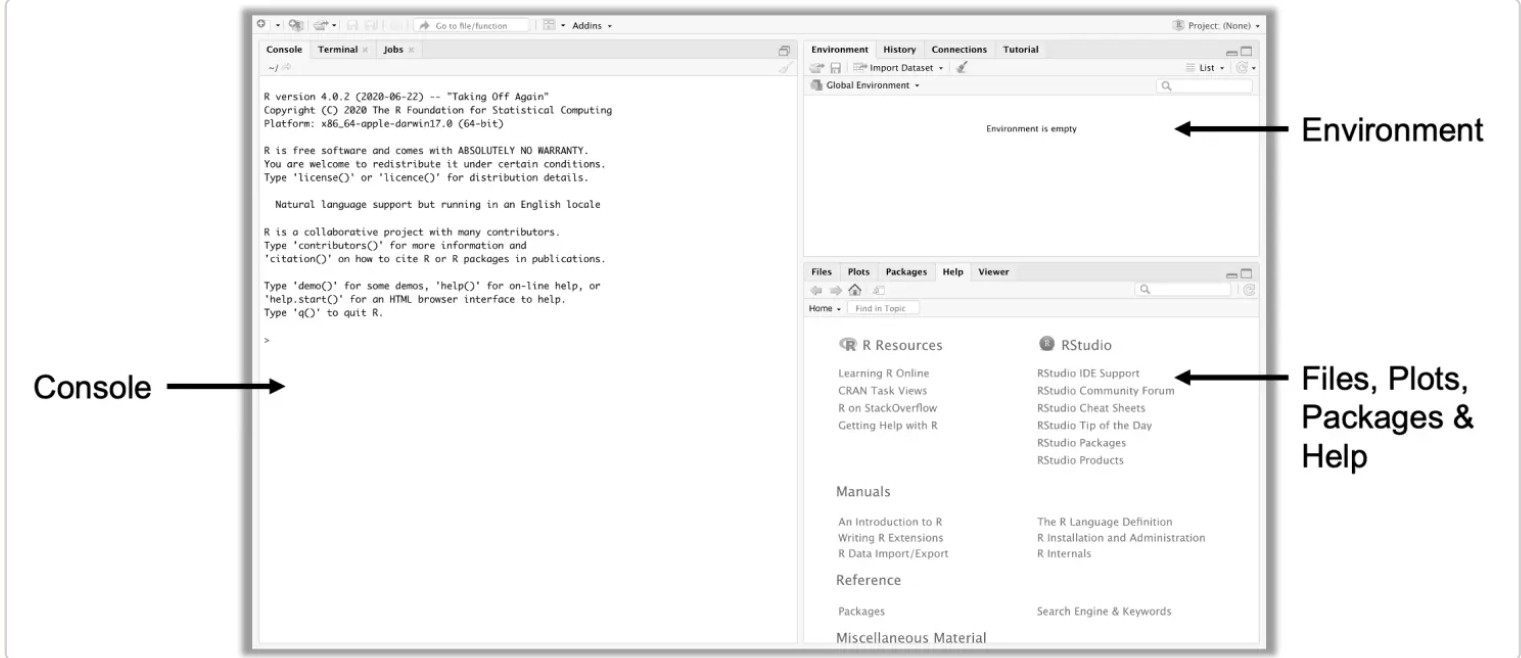
\includegraphics{C:/Users/ASUS/Dropbox/classes/R/book/img/pane rstudio.jpg}
\caption{\citet{EvaluationRCT2023}}
\end{figure}

\subsection{Understanding the RStudio Interface}\label{understanding-the-rstudio-interface}

When you first open RStudio, you'll encounter three main sections:

\begin{itemize}
\item
  \textbf{Console} :This is where the actual work happens in R. You can type R commands directly here and press Enter to execute them. Think of it as R's command center.
\item
  \textbf{Environment}: Shows all your current R objects (variables, data, functions) like a workspace overview where you can see everything you've created.
\item
  \textbf{Files/Plots/Packages/Help}: a multi-purpose area that shows: your computer's files and folders, graphs and visualizations you create, installed R packages, help documentation.
\item
  \textbf{Editor} : opens when you create a new R script (File \textgreater{} New File \textgreater{} R Script). This is where you write and save your R code Files are saved with a .R extension.
  *To run code from the editor: Select the code you want to run; Click the ``Run'' button (▹) in the top-right of the editor Or use the shortcut Ctrl+Enter (Windows) / Cmd+Enter (Mac)
\end{itemize}

\textbf{Note}: While you write code in the editor, it always executes in the console. Think of the editor as your notebook and the console as where the actual computation happens.

\section{Support and Resources}\label{support-and-resources}

\begin{itemize}
\tightlist
\item
  Office number: 404
\item
  Office hours: 8AM-8PM
\item
  Email: \href{mailto:habibou.ibrahim_kassoum@doctorant.uca.fr}{\nolinkurl{habibou.ibrahim\_kassoum@doctorant.uca.fr}}
\item
  Online forum for questions and discussions (stackoverflow)
\end{itemize}

Some online resources and reading materials:
- \href{https://bookdown.org/}{Bookdown}

\begin{itemize}
\item
  \href{https://rct-tutorial.mharrer.dev/preparation}{Evaluation of Randomized Controlled Trials With R}
\item
  \href{https://pierrebeaucoral.github.io/course/r-for-beginners/CoursR.html\#course-outline}{Pierre Beaucoral's classes}
\end{itemize}

Remember, learning to program is like learning a new language - it takes practice and patience. Don't hesitate to ask questions and collaborate with your peers throughout this journey.

Let's begin this exciting journey into the world of R programming for health economics!

\chapter{R basic data manipulations}\label{r-basic-data-manipulations}

\section{Introduction to R Syntax}\label{introduction-to-r-syntax}

R is a powerful programming language designed specifically for statistical computing and data analysis. Let's explore its fundamental concepts.

\subsection{Variables and Data Types}\label{variables-and-data-types}

Before diving into coding, it's essential to understand the basic data types in R. Think of variables as containers that store different types of information. R has three main types of data that you'll use frequently:

\begin{Shaded}
\begin{Highlighting}[]
\CommentTok{\# Numeric (integers and decimals)}
\CommentTok{\# Numbers can be whole (integers) or have decimal points}
\NormalTok{my\_number }\OtherTok{\textless{}{-}} \FloatTok{42.5}
\FunctionTok{print}\NormalTok{(my\_number)}
\end{Highlighting}
\end{Shaded}

\begin{verbatim}
## [1] 42.5
\end{verbatim}

\begin{Shaded}
\begin{Highlighting}[]
\CommentTok{\# Character (text strings)}
\CommentTok{\# Any text data must be enclosed in quotes}
\NormalTok{my\_text }\OtherTok{\textless{}{-}} \StringTok{"Hello R Markdown!"}
\FunctionTok{print}\NormalTok{(my\_text)}
\end{Highlighting}
\end{Shaded}

\begin{verbatim}
## [1] "Hello R Markdown!"
\end{verbatim}

\begin{Shaded}
\begin{Highlighting}[]
\CommentTok{\# Logical (boolean values)}
\CommentTok{\# TRUE/FALSE values are useful for conditional operations}
\NormalTok{my\_logical }\OtherTok{\textless{}{-}} \ConstantTok{TRUE}
\FunctionTok{print}\NormalTok{(my\_logical)}
\end{Highlighting}
\end{Shaded}

\begin{verbatim}
## [1] TRUE
\end{verbatim}

The \emph{\textless-} symbol is the assignment operator in R. While you can use \emph{=}, \emph{\textless-} is preferred in the R community. Let's practice creating meaningful variables:

\begin{Shaded}
\begin{Highlighting}[]
\CommentTok{\# Create and assign variables}
\NormalTok{age }\OtherTok{\textless{}{-}} \DecValTok{25}        \CommentTok{\# Numeric}
\NormalTok{name }\OtherTok{\textless{}{-}} \StringTok{"Alice"}  \CommentTok{\# Character}
\NormalTok{is\_student }\OtherTok{\textless{}{-}} \ConstantTok{TRUE}  \CommentTok{\# Logical}

\CommentTok{\# Display our variables}
\FunctionTok{print}\NormalTok{(age)}
\end{Highlighting}
\end{Shaded}

\begin{verbatim}
## [1] 25
\end{verbatim}

\begin{Shaded}
\begin{Highlighting}[]
\FunctionTok{print}\NormalTok{(name)}
\end{Highlighting}
\end{Shaded}

\begin{verbatim}
## [1] "Alice"
\end{verbatim}

\begin{Shaded}
\begin{Highlighting}[]
\FunctionTok{print}\NormalTok{(is\_student)}
\end{Highlighting}
\end{Shaded}

\begin{verbatim}
## [1] TRUE
\end{verbatim}

\begin{Shaded}
\begin{Highlighting}[]
\CommentTok{\# Check variable types using class()}
\CommentTok{\# This is useful to confirm what type of data you\textquotesingle{}re working with}
\FunctionTok{class}\NormalTok{(age)}
\end{Highlighting}
\end{Shaded}

\begin{verbatim}
## [1] "numeric"
\end{verbatim}

\begin{Shaded}
\begin{Highlighting}[]
\FunctionTok{class}\NormalTok{(name)}
\end{Highlighting}
\end{Shaded}

\begin{verbatim}
## [1] "character"
\end{verbatim}

\begin{Shaded}
\begin{Highlighting}[]
\FunctionTok{class}\NormalTok{(is\_student)}
\end{Highlighting}
\end{Shaded}

\begin{verbatim}
## [1] "logical"
\end{verbatim}

\subsection{Basic Operations}\label{basic-operations}

R can perform various arithmetic operations just like a calculator. These operations are fundamental to data analysis: addition, subtraction, multiplication, division

\begin{Shaded}
\begin{Highlighting}[]
\CommentTok{\# Basic arithmetic operations are straightforward}
\NormalTok{addition }\OtherTok{\textless{}{-}} \DecValTok{10} \SpecialCharTok{+} \DecValTok{5}       \CommentTok{\# Adding numbers}
\NormalTok{subtraction }\OtherTok{\textless{}{-}} \DecValTok{10} \SpecialCharTok{{-}} \DecValTok{5}    \CommentTok{\# Subtracting numbers}
\NormalTok{multiplication }\OtherTok{\textless{}{-}} \DecValTok{10} \SpecialCharTok{*} \DecValTok{5} \CommentTok{\# Multiplying numbers}
\NormalTok{division }\OtherTok{\textless{}{-}} \DecValTok{10} \SpecialCharTok{/} \DecValTok{5}       \CommentTok{\# Dividing numbers}

\CommentTok{\# Display results}
\FunctionTok{print}\NormalTok{(addition)}
\end{Highlighting}
\end{Shaded}

\begin{verbatim}
## [1] 15
\end{verbatim}

\begin{Shaded}
\begin{Highlighting}[]
\FunctionTok{print}\NormalTok{(subtraction)}
\end{Highlighting}
\end{Shaded}

\begin{verbatim}
## [1] 5
\end{verbatim}

\begin{Shaded}
\begin{Highlighting}[]
\FunctionTok{print}\NormalTok{(multiplication)}
\end{Highlighting}
\end{Shaded}

\begin{verbatim}
## [1] 50
\end{verbatim}

\begin{Shaded}
\begin{Highlighting}[]
\FunctionTok{print}\NormalTok{(division)}
\end{Highlighting}
\end{Shaded}

\begin{verbatim}
## [1] 2
\end{verbatim}

\begin{Shaded}
\begin{Highlighting}[]
\CommentTok{\# More complex mathematical operations}
\NormalTok{power }\OtherTok{\textless{}{-}} \DecValTok{2}\SpecialCharTok{\^{}}\DecValTok{3}            \CommentTok{\# Exponentiation (2 to the power of 3)}
\NormalTok{square\_root }\OtherTok{\textless{}{-}} \FunctionTok{sqrt}\NormalTok{(}\DecValTok{16}\NormalTok{) }\CommentTok{\# Square root function}
\FunctionTok{print}\NormalTok{(power)}
\end{Highlighting}
\end{Shaded}

\begin{verbatim}
## [1] 8
\end{verbatim}

\begin{Shaded}
\begin{Highlighting}[]
\FunctionTok{print}\NormalTok{(square\_root)}
\end{Highlighting}
\end{Shaded}

\begin{verbatim}
## [1] 4
\end{verbatim}

Logical operations are crucial for data filtering and conditional statements:

\begin{Shaded}
\begin{Highlighting}[]
\CommentTok{\# Comparison operators return TRUE or FALSE}
\NormalTok{equals }\OtherTok{\textless{}{-}} \DecValTok{5} \SpecialCharTok{==} \DecValTok{5}        \CommentTok{\# Equality comparison}
\NormalTok{greater\_than }\OtherTok{\textless{}{-}} \DecValTok{10} \SpecialCharTok{\textgreater{}} \DecValTok{5}  \CommentTok{\# Greater than comparison}
\NormalTok{less\_than }\OtherTok{\textless{}{-}} \DecValTok{3} \SpecialCharTok{\textless{}} \DecValTok{7}     \CommentTok{\# Less than comparison}

\CommentTok{\# Logical operators combine TRUE/FALSE values}
\NormalTok{and\_operator }\OtherTok{\textless{}{-}} \ConstantTok{TRUE} \SpecialCharTok{\&} \ConstantTok{TRUE}    \CommentTok{\# Both conditions must be TRUE}
\NormalTok{or\_operator }\OtherTok{\textless{}{-}} \ConstantTok{TRUE} \SpecialCharTok{|} \ConstantTok{FALSE}    \CommentTok{\# At least one condition must be TRUE}

\CommentTok{\# Print results}
\FunctionTok{print}\NormalTok{(equals)}
\end{Highlighting}
\end{Shaded}

\begin{verbatim}
## [1] TRUE
\end{verbatim}

\begin{Shaded}
\begin{Highlighting}[]
\FunctionTok{print}\NormalTok{(greater\_than)}
\end{Highlighting}
\end{Shaded}

\begin{verbatim}
## [1] TRUE
\end{verbatim}

\begin{Shaded}
\begin{Highlighting}[]
\FunctionTok{print}\NormalTok{(less\_than)}
\end{Highlighting}
\end{Shaded}

\begin{verbatim}
## [1] TRUE
\end{verbatim}

\begin{Shaded}
\begin{Highlighting}[]
\FunctionTok{print}\NormalTok{(and\_operator)}
\end{Highlighting}
\end{Shaded}

\begin{verbatim}
## [1] TRUE
\end{verbatim}

\begin{Shaded}
\begin{Highlighting}[]
\FunctionTok{print}\NormalTok{(or\_operator)}
\end{Highlighting}
\end{Shaded}

\begin{verbatim}
## [1] TRUE
\end{verbatim}

\section{Objects in R}\label{objects-in-r}

\begin{figure}
\centering
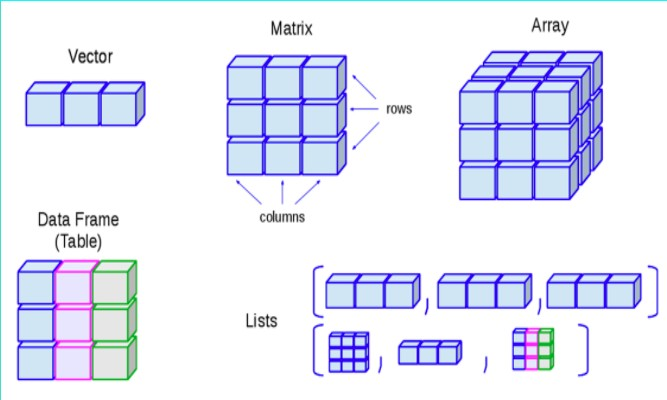
\includegraphics{C:/Users/ASUS/Dropbox/classes/R/book/img/object_list R.jpg}
\caption{(image from \url{http://venus.ifca.unican.es/Rintro/dataStruct.html})}
\end{figure}

\subsection{Working with Vectors}\label{working-with-vectors}

Vectors are one of the most basic data structures in R. Think of them as a collection of elements of the same type, like a list of numbers or strings:

\begin{Shaded}
\begin{Highlighting}[]
\CommentTok{\# Creating vectors using the combine function c()}
\NormalTok{numeric\_vector }\OtherTok{\textless{}{-}} \FunctionTok{c}\NormalTok{(}\DecValTok{1}\NormalTok{, }\DecValTok{2}\NormalTok{, }\DecValTok{3}\NormalTok{, }\DecValTok{4}\NormalTok{, }\DecValTok{5}\NormalTok{)           }\CommentTok{\# Vector of numbers}
\NormalTok{character\_vector }\OtherTok{\textless{}{-}} \FunctionTok{c}\NormalTok{(}\StringTok{"apple"}\NormalTok{, }\StringTok{"banana"}\NormalTok{, }\StringTok{"cherry"}\NormalTok{, }\StringTok{"avocado"}\NormalTok{, }\StringTok{"mango"}\NormalTok{)  }\CommentTok{\# Vector of strings}
\NormalTok{logical\_vector }\OtherTok{\textless{}{-}} \FunctionTok{c}\NormalTok{(}\ConstantTok{TRUE}\NormalTok{, }\ConstantTok{FALSE}\NormalTok{, }\ConstantTok{TRUE}\NormalTok{)       }\CommentTok{\# Vector of logical values}

\CommentTok{\# Display vectors}
\FunctionTok{print}\NormalTok{(numeric\_vector)}
\end{Highlighting}
\end{Shaded}

\begin{verbatim}
## [1] 1 2 3 4 5
\end{verbatim}

\begin{Shaded}
\begin{Highlighting}[]
\FunctionTok{print}\NormalTok{(character\_vector)}
\end{Highlighting}
\end{Shaded}

\begin{verbatim}
## [1] "apple"   "banana"  "cherry"  "avocado" "mango"
\end{verbatim}

\begin{Shaded}
\begin{Highlighting}[]
\FunctionTok{print}\NormalTok{(logical\_vector)}
\end{Highlighting}
\end{Shaded}

\begin{verbatim}
## [1]  TRUE FALSE  TRUE
\end{verbatim}

\begin{Shaded}
\begin{Highlighting}[]
\CommentTok{\# Vector operations {-} R can perform operations on entire vectors at once}
\CommentTok{\# This is called vectorization and is very efficient}
\FunctionTok{print}\NormalTok{(}\FunctionTok{length}\NormalTok{(numeric\_vector)) }\CommentTok{\# length of the vector}
\end{Highlighting}
\end{Shaded}

\begin{verbatim}
## [1] 5
\end{verbatim}

\begin{Shaded}
\begin{Highlighting}[]
\NormalTok{doubled }\OtherTok{\textless{}{-}}\NormalTok{ numeric\_vector }\SpecialCharTok{*} \DecValTok{2}  \CommentTok{\# Multiply each element by 2}
\FunctionTok{print}\NormalTok{(doubled)}
\end{Highlighting}
\end{Shaded}

\begin{verbatim}
## [1]  2  4  6  8 10
\end{verbatim}

\begin{Shaded}
\begin{Highlighting}[]
\CommentTok{\# Accessing elements using indexing}
\CommentTok{\# R uses 1{-}based indexing (first element is at position 1, not 0)}
\NormalTok{first\_element }\OtherTok{\textless{}{-}}\NormalTok{ numeric\_vector[}\DecValTok{1}\NormalTok{]  }\CommentTok{\# Get first element}
\NormalTok{selected\_elements }\OtherTok{\textless{}{-}}\NormalTok{ numeric\_vector[}\FunctionTok{c}\NormalTok{(}\DecValTok{1}\NormalTok{, }\DecValTok{3}\NormalTok{, }\DecValTok{5}\NormalTok{)]  }\CommentTok{\# Get specific elements}
\FunctionTok{print}\NormalTok{(first\_element)}
\end{Highlighting}
\end{Shaded}

\begin{verbatim}
## [1] 1
\end{verbatim}

\begin{Shaded}
\begin{Highlighting}[]
\FunctionTok{print}\NormalTok{(selected\_elements)}
\end{Highlighting}
\end{Shaded}

\begin{verbatim}
## [1] 1 3 5
\end{verbatim}

\subsection{Creating Sequences}\label{creating-sequences}

R provides several convenient ways to create sequences of numbers, which is particularly useful for data analysis and plotting:

\begin{Shaded}
\begin{Highlighting}[]
\CommentTok{\# Using seq() for more control over sequence generation}
\NormalTok{sequence1 }\OtherTok{\textless{}{-}} \FunctionTok{seq}\NormalTok{(}\DecValTok{1}\NormalTok{, }\DecValTok{10}\NormalTok{)          }\CommentTok{\# Basic sequence from 1 to 10}
\NormalTok{sequence2 }\OtherTok{\textless{}{-}} \FunctionTok{seq}\NormalTok{(}\DecValTok{0}\NormalTok{, }\DecValTok{20}\NormalTok{, }\AttributeTok{by =} \DecValTok{2}\NormalTok{)  }\CommentTok{\# Even numbers from 0 to 20}

\CommentTok{\# Using : operator for simple sequences}
\NormalTok{sequence3 }\OtherTok{\textless{}{-}} \DecValTok{1}\SpecialCharTok{:}\DecValTok{10}                \CommentTok{\# Another way to create sequence from 1 to 10}

\CommentTok{\# Using rep() to repeat values}
\NormalTok{repeated }\OtherTok{\textless{}{-}} \FunctionTok{rep}\NormalTok{(}\DecValTok{5}\NormalTok{, }\AttributeTok{times =} \DecValTok{3}\NormalTok{)    }\CommentTok{\# Repeat the number 5 three times}

\FunctionTok{print}\NormalTok{(sequence1)}
\end{Highlighting}
\end{Shaded}

\begin{verbatim}
##  [1]  1  2  3  4  5  6  7  8  9 10
\end{verbatim}

\begin{Shaded}
\begin{Highlighting}[]
\FunctionTok{print}\NormalTok{(sequence2)}
\end{Highlighting}
\end{Shaded}

\begin{verbatim}
##  [1]  0  2  4  6  8 10 12 14 16 18 20
\end{verbatim}

\begin{Shaded}
\begin{Highlighting}[]
\FunctionTok{print}\NormalTok{(sequence3)}
\end{Highlighting}
\end{Shaded}

\begin{verbatim}
##  [1]  1  2  3  4  5  6  7  8  9 10
\end{verbatim}

\begin{Shaded}
\begin{Highlighting}[]
\FunctionTok{print}\NormalTok{(repeated)}
\end{Highlighting}
\end{Shaded}

\begin{verbatim}
## [1] 5 5 5
\end{verbatim}

\section{Exercise 1}\label{exercise-1}

\textbf{Understanding Data Types}

Create three variables and assign them values of different data types:

\begin{itemize}
\tightlist
\item
  A numeric variable representing your height in centimeters.
\item
  A character variable storing your favorite fruit.
\item
  A logical variable indicating whether you like R programming.
\end{itemize}

Then, print each variable and use class() to check its data type.

\textbf{Basic Arithmetic Operations}

Perform the following calculations and store the results in variables:

\begin{itemize}
\tightlist
\item
  Multiply 15 by 3.
\item
  Subtract 7 from 100.
\item
  Compute the square root of 64.
\item
  Raise 3 to the power of 4.
\end{itemize}

Print all results.

\textbf{Vector Manipulation}

\begin{itemize}
\item
  Create a numeric vector containing the numbers 2, 4, 6, 8, 10. Multiply all elements of the vector by 3. Extract the second and fourth elements of the vector.
\item
  Create a character vector with three country names of your choice. Multiply it by 3.
\end{itemize}

\textbf{Creating Sequences}

\begin{itemize}
\tightlist
\item
  Create a sequence of numbers from 5 to 50 with a step size of 5.
\item
  Generate a sequence of odd numbers from 1 to 15 using seq().
\item
  Use rep() to create a vector that repeats the number 7 five times.
\end{itemize}

\subsection{Working with Data Frames}\label{working-with-data-frames}

Data frames are the most common way to work with structured data in R. They're similar to Excel spreadsheets or database tables:

\begin{Shaded}
\begin{Highlighting}[]
\CommentTok{\# Create a simple data frame}
\CommentTok{\# Each column can have a different data type}
\NormalTok{students\_df }\OtherTok{\textless{}{-}} \FunctionTok{data.frame}\NormalTok{(}
  \AttributeTok{name =} \FunctionTok{c}\NormalTok{(}\StringTok{"Monelson"}\NormalTok{, }\StringTok{"Noemie"}\NormalTok{, }\StringTok{"Alphonse"}\NormalTok{, }\StringTok{"Aichatou"}\NormalTok{, }\StringTok{"Laurene"}\NormalTok{, }\StringTok{"Anonkoua"}\NormalTok{),    }\CommentTok{\# Character column}
  \AttributeTok{age =} \FunctionTok{c}\NormalTok{(}\DecValTok{25}\NormalTok{, }\DecValTok{20}\NormalTok{, }\DecValTok{23}\NormalTok{, }\DecValTok{22}\NormalTok{, }\DecValTok{22}\NormalTok{, }\DecValTok{26}\NormalTok{),                    }\CommentTok{\# Numeric column}
  \AttributeTok{note =} \FunctionTok{c}\NormalTok{(}\DecValTok{10}\NormalTok{, }\DecValTok{15}\NormalTok{, }\DecValTok{13}\NormalTok{, }\DecValTok{15}\NormalTok{, }\FloatTok{16.5}\NormalTok{, }\DecValTok{9}\NormalTok{),                 }\CommentTok{\# Numeric column}
  \AttributeTok{is\_graduate =} \FunctionTok{c}\NormalTok{(}\ConstantTok{FALSE}\NormalTok{, }\ConstantTok{TRUE}\NormalTok{, }\ConstantTok{TRUE}\NormalTok{, }\ConstantTok{TRUE}\NormalTok{, T, F)      }\CommentTok{\# Logical column}
\NormalTok{)}

\CommentTok{\# Display the data frame}
\FunctionTok{print}\NormalTok{(students\_df)}
\end{Highlighting}
\end{Shaded}

\begin{verbatim}
##       name age note is_graduate
## 1 Monelson  25 10.0       FALSE
## 2   Noemie  20 15.0        TRUE
## 3 Alphonse  23 13.0        TRUE
## 4 Aichatou  22 15.0        TRUE
## 5  Laurene  22 16.5        TRUE
## 6 Anonkoua  26  9.0       FALSE
\end{verbatim}

\begin{Shaded}
\begin{Highlighting}[]
\CommentTok{\# Basic data frame operations}
\CommentTok{\# Access a column using $ notation}
\FunctionTok{print}\NormalTok{(students\_df}\SpecialCharTok{$}\NormalTok{age)}
\end{Highlighting}
\end{Shaded}

\begin{verbatim}
## [1] 25 20 23 22 22 26
\end{verbatim}

\begin{Shaded}
\begin{Highlighting}[]
\CommentTok{\# Access a row using index}
\FunctionTok{print}\NormalTok{(students\_df[}\DecValTok{5}\NormalTok{, ])}
\end{Highlighting}
\end{Shaded}

\begin{verbatim}
##      name age note is_graduate
## 5 Laurene  22 16.5        TRUE
\end{verbatim}

\begin{Shaded}
\begin{Highlighting}[]
\CommentTok{\# Add a new column {-} must match the number of rows}
\NormalTok{students\_df}\SpecialCharTok{$}\NormalTok{height }\OtherTok{\textless{}{-}} \FunctionTok{c}\NormalTok{(}\DecValTok{175}\NormalTok{, }\DecValTok{168}\NormalTok{, }\DecValTok{182}\NormalTok{, }\DecValTok{150}\NormalTok{, }\DecValTok{160}\NormalTok{, }\DecValTok{155}\NormalTok{)}
\FunctionTok{print}\NormalTok{(students\_df)}
\end{Highlighting}
\end{Shaded}

\begin{verbatim}
##       name age note is_graduate height
## 1 Monelson  25 10.0       FALSE    175
## 2   Noemie  20 15.0        TRUE    168
## 3 Alphonse  23 13.0        TRUE    182
## 4 Aichatou  22 15.0        TRUE    150
## 5  Laurene  22 16.5        TRUE    160
## 6 Anonkoua  26  9.0       FALSE    155
\end{verbatim}

\section{Importing an Manipulating data in R}\label{importing-an-manipulating-data-in-r}

\subsection{Importing data}\label{importing-data}

\begin{Shaded}
\begin{Highlighting}[]
\CommentTok{\# Installing and Loading the Required Package}

\DocumentationTok{\#\# First, install and load the \textasciigrave{}medicaldata\textasciigrave{} package to access the \textasciigrave{}covid\_testing\textasciigrave{} dataset.}


\CommentTok{\# Install the package (only needs to be done once)}
\DocumentationTok{\#\# install.packages("medicaldata")}

\CommentTok{\# Load the package into the R session}
\FunctionTok{library}\NormalTok{(}\StringTok{"medicaldata"}\NormalTok{)}

\CommentTok{\# Load the COVID{-}19 testing dataset from the medicaldata package}
\NormalTok{covid }\OtherTok{\textless{}{-}}\NormalTok{ medicaldata}\SpecialCharTok{::}\NormalTok{covid\_testing}

\CommentTok{\# Display the first few rows of the dataset}
\FunctionTok{head}\NormalTok{(covid)}
\end{Highlighting}
\end{Shaded}

\begin{verbatim}
##   subject_id fake_first_name fake_last_name gender pan_day test_id
## 1       1412         jhezane     westerling female       4   covid
## 2        533           penny      targaryen female       7   covid
## 3       9134           grunt         rivers   male       7   covid
## 4       8518      melisandre          swyft female       8   covid
## 5       8967          rolley       karstark   male       8   covid
## 6      11048           megga       karstark female       8   covid
##         clinic_name   result demo_group age drive_thru_ind ct_result orderset
## 1  inpatient ward a negative    patient 0.0              0        45        0
## 2      clinical lab negative    patient 0.0              1        45        0
## 3      clinical lab negative    patient 0.8              1        45        1
## 4      clinical lab negative    patient 0.8              1        45        1
## 5    emergency dept negative    patient 0.8              0        45        1
## 6 oncology day hosp negative    patient 0.8              0        45        0
##   payor_group        patient_class col_rec_tat rec_ver_tat
## 1  government            inpatient         1.4         5.2
## 2  commercial       not applicable         2.3         5.8
## 3        <NA>                 <NA>         7.3         4.7
## 4        <NA>                 <NA>         5.8         5.0
## 5  government            emergency         1.2         6.4
## 6  commercial recurring outpatient         1.4         7.0
\end{verbatim}

\begin{Shaded}
\begin{Highlighting}[]
\CommentTok{\# Show the column names of the dataset}
\FunctionTok{colnames}\NormalTok{(covid)   }
\end{Highlighting}
\end{Shaded}

\begin{verbatim}
##  [1] "subject_id"      "fake_first_name" "fake_last_name"  "gender"         
##  [5] "pan_day"         "test_id"         "clinic_name"     "result"         
##  [9] "demo_group"      "age"             "drive_thru_ind"  "ct_result"      
## [13] "orderset"        "payor_group"     "patient_class"   "col_rec_tat"    
## [17] "rec_ver_tat"
\end{verbatim}

\begin{Shaded}
\begin{Highlighting}[]
\CommentTok{\# Show the number of columns in the dataset}
\FunctionTok{ncol}\NormalTok{(covid)       }
\end{Highlighting}
\end{Shaded}

\begin{verbatim}
## [1] 17
\end{verbatim}

\begin{Shaded}
\begin{Highlighting}[]
\CommentTok{\# Show the number of rows in the dataset}
\FunctionTok{nrow}\NormalTok{(covid)    }
\end{Highlighting}
\end{Shaded}

\begin{verbatim}
## [1] 15524
\end{verbatim}

\subsection{Data Frame Manipulation}\label{data-frame-manipulation}

Data frames support powerful operations for data analysis:

\begin{Shaded}
\begin{Highlighting}[]
\CommentTok{\# Filter data based on conditions}
\NormalTok{high\_gpa }\OtherTok{\textless{}{-}}\NormalTok{ students\_df[students\_df}\SpecialCharTok{$}\NormalTok{gpa }\SpecialCharTok{\textgreater{}} \FloatTok{3.5}\NormalTok{, ]  }\CommentTok{\# Select rows where GPA \textgreater{} 3.5}
\FunctionTok{print}\NormalTok{(high\_gpa)}
\end{Highlighting}
\end{Shaded}

\begin{verbatim}
## [1] name        age         note        is_graduate height     
## <0 lignes> (ou 'row.names' de longueur nulle)
\end{verbatim}

\begin{Shaded}
\begin{Highlighting}[]
\CommentTok{\# Sort data using order()}
\NormalTok{sorted\_by\_age }\OtherTok{\textless{}{-}}\NormalTok{ students\_df[}\FunctionTok{order}\NormalTok{(students\_df}\SpecialCharTok{$}\NormalTok{age), ]  }\CommentTok{\# Sort by age}
\FunctionTok{print}\NormalTok{(sorted\_by\_age)}
\end{Highlighting}
\end{Shaded}

\begin{verbatim}
##       name age note is_graduate height
## 2   Noemie  20 15.0        TRUE    168
## 4 Aichatou  22 15.0        TRUE    150
## 5  Laurene  22 16.5        TRUE    160
## 3 Alphonse  23 13.0        TRUE    182
## 1 Monelson  25 10.0       FALSE    175
## 6 Anonkoua  26  9.0       FALSE    155
\end{verbatim}

\begin{Shaded}
\begin{Highlighting}[]
\CommentTok{\# Or}

\FunctionTok{sort}\NormalTok{(students\_df}\SpecialCharTok{$}\NormalTok{age)}
\end{Highlighting}
\end{Shaded}

\begin{verbatim}
## [1] 20 22 22 23 25 26
\end{verbatim}

\section{Exercise 2}\label{exercise-2}

\begin{itemize}
\item
  Import the \textbf{``blood\_storage''} database from the package \textbf{medicaldata}.
\item
  Log-transform the variable \emph{age} in data and save the result as \emph{age.log}.
\item
  Square all values in \emph{PVol} (Prostate
  ~volume) and save the result as \emph{PVol.squared} within the dataset.
\item
  Check whether the \emph{AA} (African American race) is of class factor (0 = ``non‐African-American''; 1 = ``African American'').
\item
  Filter out the records for which \emph{(PreopPSA \textgreater= 10)} and \emph{(Recurrence == 0)}.
\item
  In the \emph{fifth} and \emph{sixth} rows of the data, change the value of \emph{Age} to NA (missing).
\item
  Remove the variables from the dataset: \emph{AA},\emph{FamHx},\emph{OrganConfined}.
\end{itemize}

Remember that R is case-sensitive and very particular about syntax. Pay attention to brackets, commas, and quotation marks. The best way to learn is by experimenting with the code and modifying it to see what happens!

\chapter{Data Wrangling and basic statistics}\label{data-wrangling-and-basic-statistics}

\section{1. Introduction to dplyr}\label{introduction-to-dplyr}

The \texttt{dplyr} package is a powerful tool in R for data manipulation. It provides functions for filtering, selecting, arranging, summarizing, and mutating data in an easy and readable way. The \texttt{\%\textgreater{}\%} (pipe operator) is commonly used to link functions together.

\begin{Shaded}
\begin{Highlighting}[]
\CommentTok{\# Install and load necessary packages}
\CommentTok{\#install.packages("dplyr")}
\CommentTok{\#install.packages("medicaldata")}

\FunctionTok{library}\NormalTok{(dplyr)}
\end{Highlighting}
\end{Shaded}

\begin{verbatim}
## 
## Attachement du package : 'dplyr'
\end{verbatim}

\begin{verbatim}
## Les objets suivants sont masqués depuis 'package:stats':
## 
##     filter, lag
\end{verbatim}

\begin{verbatim}
## Les objets suivants sont masqués depuis 'package:base':
## 
##     intersect, setdiff, setequal, union
\end{verbatim}

\begin{Shaded}
\begin{Highlighting}[]
\FunctionTok{library}\NormalTok{(medicaldata)}

\CommentTok{\# Print all the function in the package dplyr}
\FunctionTok{ls}\NormalTok{(}\StringTok{"package:dplyr"}\NormalTok{)}
\end{Highlighting}
\end{Shaded}

\begin{verbatim}
##   [1] "%>%"                   "across"                "add_count"            
##   [4] "add_count_"            "add_row"               "add_rownames"         
##   [7] "add_tally"             "add_tally_"            "all_equal"            
##  [10] "all_of"                "all_vars"              "anti_join"            
##  [13] "any_of"                "any_vars"              "arrange"              
##  [16] "arrange_"              "arrange_all"           "arrange_at"           
##  [19] "arrange_if"            "as.tbl"                "as_data_frame"        
##  [22] "as_label"              "as_tibble"             "auto_copy"            
##  [25] "band_instruments"      "band_instruments2"     "band_members"         
##  [28] "bench_tbls"            "between"               "bind_cols"            
##  [31] "bind_rows"             "c_across"              "case_match"           
##  [34] "case_when"             "changes"               "check_dbplyr"         
##  [37] "coalesce"              "collapse"              "collect"              
##  [40] "combine"               "common_by"             "compare_tbls"         
##  [43] "compare_tbls2"         "compute"               "consecutive_id"       
##  [46] "contains"              "copy_to"               "count"                
##  [49] "count_"                "cross_join"            "cumall"               
##  [52] "cumany"                "cume_dist"             "cummean"              
##  [55] "cur_column"            "cur_data"              "cur_data_all"         
##  [58] "cur_group"             "cur_group_id"          "cur_group_rows"       
##  [61] "current_vars"          "data_frame"            "db_analyze"           
##  [64] "db_begin"              "db_commit"             "db_create_index"      
##  [67] "db_create_indexes"     "db_create_table"       "db_data_type"         
##  [70] "db_desc"               "db_drop_table"         "db_explain"           
##  [73] "db_has_table"          "db_insert_into"        "db_list_tables"       
##  [76] "db_query_fields"       "db_query_rows"         "db_rollback"          
##  [79] "db_save_query"         "db_write_table"        "dense_rank"           
##  [82] "desc"                  "dim_desc"              "distinct"             
##  [85] "distinct_"             "distinct_all"          "distinct_at"          
##  [88] "distinct_if"           "distinct_prepare"      "do"                   
##  [91] "do_"                   "dplyr_col_modify"      "dplyr_reconstruct"    
##  [94] "dplyr_row_slice"       "ends_with"             "enexpr"               
##  [97] "enexprs"               "enquo"                 "enquos"               
## [100] "ensym"                 "ensyms"                "eval_tbls"            
## [103] "eval_tbls2"            "everything"            "explain"              
## [106] "expr"                  "failwith"              "filter"               
## [109] "filter_"               "filter_all"            "filter_at"            
## [112] "filter_if"             "first"                 "full_join"            
## [115] "funs"                  "funs_"                 "glimpse"              
## [118] "group_by"              "group_by_"             "group_by_all"         
## [121] "group_by_at"           "group_by_drop_default" "group_by_if"          
## [124] "group_by_prepare"      "group_cols"            "group_data"           
## [127] "group_indices"         "group_indices_"        "group_keys"           
## [130] "group_map"             "group_modify"          "group_nest"           
## [133] "group_rows"            "group_size"            "group_split"          
## [136] "group_trim"            "group_vars"            "group_walk"           
## [139] "grouped_df"            "groups"                "id"                   
## [142] "ident"                 "if_all"                "if_any"               
## [145] "if_else"               "inner_join"            "intersect"            
## [148] "is.grouped_df"         "is.src"                "is.tbl"               
## [151] "is_grouped_df"         "join_by"               "lag"                  
## [154] "last"                  "last_col"              "last_dplyr_warnings"  
## [157] "lead"                  "left_join"             "location"             
## [160] "lst"                   "make_tbl"              "matches"              
## [163] "min_rank"              "mutate"                "mutate_"              
## [166] "mutate_all"            "mutate_at"             "mutate_each"          
## [169] "mutate_each_"          "mutate_if"             "n"                    
## [172] "n_distinct"            "n_groups"              "na_if"                
## [175] "near"                  "nest_by"               "nest_join"            
## [178] "new_grouped_df"        "new_rowwise_df"        "nth"                  
## [181] "ntile"                 "num_range"             "one_of"               
## [184] "order_by"              "percent_rank"          "pick"                 
## [187] "progress_estimated"    "pull"                  "quo"                  
## [190] "quo_name"              "quos"                  "recode"               
## [193] "recode_factor"         "reframe"               "relocate"             
## [196] "rename"                "rename_"               "rename_all"           
## [199] "rename_at"             "rename_if"             "rename_vars"          
## [202] "rename_vars_"          "rename_with"           "right_join"           
## [205] "row_number"            "rows_append"           "rows_delete"          
## [208] "rows_insert"           "rows_patch"            "rows_update"          
## [211] "rows_upsert"           "rowwise"               "same_src"             
## [214] "sample_frac"           "sample_n"              "select"               
## [217] "select_"               "select_all"            "select_at"            
## [220] "select_if"             "select_var"            "select_vars"          
## [223] "select_vars_"          "semi_join"             "setdiff"              
## [226] "setequal"              "show_query"            "slice"                
## [229] "slice_"                "slice_head"            "slice_max"            
## [232] "slice_min"             "slice_sample"          "slice_tail"           
## [235] "sql"                   "sql_escape_ident"      "sql_escape_string"    
## [238] "sql_join"              "sql_select"            "sql_semi_join"        
## [241] "sql_set_op"            "sql_subquery"          "sql_translate_env"    
## [244] "src"                   "src_df"                "src_local"            
## [247] "src_mysql"             "src_postgres"          "src_sqlite"           
## [250] "src_tbls"              "starts_with"           "starwars"             
## [253] "storms"                "summarise"             "summarise_"           
## [256] "summarise_all"         "summarise_at"          "summarise_each"       
## [259] "summarise_each_"       "summarise_if"          "summarize"            
## [262] "summarize_"            "summarize_all"         "summarize_at"         
## [265] "summarize_each"        "summarize_each_"       "summarize_if"         
## [268] "sym"                   "symdiff"               "syms"                 
## [271] "tally"                 "tally_"                "tbl"                  
## [274] "tbl_df"                "tbl_nongroup_vars"     "tbl_ptype"            
## [277] "tbl_vars"              "tibble"                "top_frac"             
## [280] "top_n"                 "transmute"             "transmute_"           
## [283] "transmute_all"         "transmute_at"          "transmute_if"         
## [286] "tribble"               "type_sum"              "ungroup"              
## [289] "union"                 "union_all"             "validate_grouped_df"  
## [292] "validate_rowwise_df"   "vars"                  "where"                
## [295] "with_groups"           "with_order"            "wrap_dbplyr_obj"
\end{verbatim}

\begin{Shaded}
\begin{Highlighting}[]
\CommentTok{\# Load the COVID{-}19 dataset}
\NormalTok{covid }\OtherTok{\textless{}{-}}\NormalTok{ medicaldata}\SpecialCharTok{::}\NormalTok{covid\_testing}
\end{Highlighting}
\end{Shaded}

\section{Filtering, Selecting, and Arranging Data}\label{filtering-selecting-and-arranging-data}

\subsection{Filtering Data}\label{filtering-data}

\subsubsection{Filtering with Multiple Conditions}\label{filtering-with-multiple-conditions}

We can filter the dataset to focus on specific conditions. For example, let's filter cases where patients tested positive for COVID-19 (result == ``positive'').

\begin{Shaded}
\begin{Highlighting}[]
\NormalTok{positive\_cases }\OtherTok{\textless{}{-}}\NormalTok{ covid }\SpecialCharTok{\%\textgreater{}\%} 
  \FunctionTok{filter}\NormalTok{(result }\SpecialCharTok{==} \StringTok{"positive"}\NormalTok{)}

\CommentTok{\# Show the first few rows of the filtered data}
\FunctionTok{head}\NormalTok{(positive\_cases)}
\end{Highlighting}
\end{Shaded}

\begin{verbatim}
## # A tibble: 6 x 17
##   subject_id fake_first_name fake_last_name gender pan_day test_id clinic_name  
##        <dbl> <chr>           <chr>          <chr>    <dbl> <chr>   <chr>        
## 1       2114 azzak           tully          male        10 covid   inpatient wa~
## 2       7240 arryk           mormont        male        11 covid   clinical lab 
## 3      11391 zei             umber          female      11 covid   s  care ntwk 
## 4        902 owen            seaworth       male        12 covid   emergency de~
## 5       2573 glendon         lannister      male        12 covid   emergency de~
## 6       5771 janna           lannister      female      12 covid   hem onc day ~
## # i 10 more variables: result <chr>, demo_group <chr>, age <dbl>,
## #   drive_thru_ind <dbl>, ct_result <dbl>, orderset <dbl>, payor_group <chr>,
## #   patient_class <chr>, col_rec_tat <dbl>, rec_ver_tat <dbl>
\end{verbatim}

\subsubsection{Filtering with multiple conditions}\label{filtering-with-multiple-conditions-1}

We can filter patients who are female (gender == ``female'') and tested positive for COVID-19.

\begin{Shaded}
\begin{Highlighting}[]
\NormalTok{female\_positive }\OtherTok{\textless{}{-}}\NormalTok{ covid }\SpecialCharTok{\%\textgreater{}\%}
  \FunctionTok{filter}\NormalTok{(gender }\SpecialCharTok{==} \StringTok{"female"}\NormalTok{, result }\SpecialCharTok{==} \StringTok{"positive"}\NormalTok{)}

\CommentTok{\# Show the first few rows of the filtered data}
\FunctionTok{head}\NormalTok{(female\_positive)}
\end{Highlighting}
\end{Shaded}

\begin{verbatim}
## # A tibble: 6 x 17
##   subject_id fake_first_name fake_last_name gender pan_day test_id clinic_name  
##        <dbl> <chr>           <chr>          <chr>    <dbl> <chr>   <chr>        
## 1      11391 zei             umber          female      11 covid   s  care ntwk 
## 2       5771 janna           lannister      female      12 covid   hem onc day ~
## 3      11381 sansa           martell        female      13 covid   clinical lab 
## 4        864 meera           westerling     female      14 covid   clinical lab 
## 5       5023 chataya         mormont        female      15 covid   emergency de~
## 6       6493 sybelle         karstark       female      16 covid   emergency de~
## # i 10 more variables: result <chr>, demo_group <chr>, age <dbl>,
## #   drive_thru_ind <dbl>, ct_result <dbl>, orderset <dbl>, payor_group <chr>,
## #   patient_class <chr>, col_rec_tat <dbl>, rec_ver_tat <dbl>
\end{verbatim}

\subsection{Selecting Specific Columns}\label{selecting-specific-columns}

If we only need a few columns, we can use \textbf{select()} to keep only the relevant ones.

\begin{Shaded}
\begin{Highlighting}[]
\NormalTok{selected\_data }\OtherTok{\textless{}{-}}\NormalTok{ covid }\SpecialCharTok{\%\textgreater{}\%}
  \FunctionTok{select}\NormalTok{(subject\_id, age, gender, result)}

\CommentTok{\# Display the selected columns}
\FunctionTok{head}\NormalTok{(selected\_data)}
\end{Highlighting}
\end{Shaded}

\begin{verbatim}
## # A tibble: 6 x 4
##   subject_id   age gender result  
##        <dbl> <dbl> <chr>  <chr>   
## 1       1412   0   female negative
## 2        533   0   female negative
## 3       9134   0.8 male   negative
## 4       8518   0.8 female negative
## 5       8967   0.8 male   negative
## 6      11048   0.8 female negative
\end{verbatim}

We can use helper functions to select columns dynamically.

\begin{Shaded}
\begin{Highlighting}[]
\NormalTok{selected\_columns }\OtherTok{\textless{}{-}}\NormalTok{ covid }\SpecialCharTok{\%\textgreater{}\%}
  \FunctionTok{select}\NormalTok{(}\FunctionTok{starts\_with}\NormalTok{(}\StringTok{"fake"}\NormalTok{), }\FunctionTok{contains}\NormalTok{(}\StringTok{"result"}\NormalTok{))}

\CommentTok{\# Display the selected columns}
\FunctionTok{head}\NormalTok{(selected\_columns)}
\end{Highlighting}
\end{Shaded}

\begin{verbatim}
## # A tibble: 6 x 4
##   fake_first_name fake_last_name result   ct_result
##   <chr>           <chr>          <chr>        <dbl>
## 1 jhezane         westerling     negative        45
## 2 penny           targaryen      negative        45
## 3 grunt           rivers         negative        45
## 4 melisandre      swyft          negative        45
## 5 rolley          karstark       negative        45
## 6 megga           karstark       negative        45
\end{verbatim}

\subsection{Modifying Values and Missing}\label{modifying-values-and-missing}

You can change a value in a column or even replace values with NA. For example, we set the \emph{``fake\_name\_last''} to NA for the 5th row.

\begin{Shaded}
\begin{Highlighting}[]
\CommentTok{\# First}

\NormalTok{covid[}\DecValTok{5}\NormalTok{, }\StringTok{"fake\_first\_name"}\NormalTok{] }\OtherTok{\textless{}{-}} \StringTok{"SAWADOGO"}
\NormalTok{covid[}\DecValTok{5}\NormalTok{, }\StringTok{"fake\_last\_name"}\NormalTok{] }\OtherTok{\textless{}{-}} \StringTok{"Laurent Benjamin"}
\NormalTok{covid[}\DecValTok{5}\NormalTok{, }\StringTok{"age"}\NormalTok{] }\OtherTok{\textless{}{-}} \DecValTok{26}
\NormalTok{covid[}\DecValTok{5}\NormalTok{, }\StringTok{"result"}\NormalTok{] }\OtherTok{\textless{}{-}} \StringTok{"positive"}


\NormalTok{covid[}\DecValTok{6}\NormalTok{, }\StringTok{"fake\_first\_name"}\NormalTok{] }\OtherTok{\textless{}{-}} \StringTok{"OUATTARA Siguissongui"}
\NormalTok{covid[}\DecValTok{6}\NormalTok{, }\StringTok{"fake\_last\_name"}\NormalTok{] }\OtherTok{\textless{}{-}} \StringTok{"Sarah"}
\NormalTok{covid[}\DecValTok{6}\NormalTok{, }\StringTok{"age"}\NormalTok{] }\OtherTok{\textless{}{-}} \ConstantTok{NA}
\NormalTok{covid[}\DecValTok{6}\NormalTok{, }\StringTok{"result"}\NormalTok{] }\OtherTok{\textless{}{-}} \StringTok{"positive"}


\CommentTok{\# Display the selected columns}
\FunctionTok{head}\NormalTok{(covid, }\DecValTok{7}\NormalTok{)}
\end{Highlighting}
\end{Shaded}

\begin{verbatim}
## # A tibble: 7 x 17
##   subject_id fake_first_name   fake_last_name gender pan_day test_id clinic_name
##        <dbl> <chr>             <chr>          <chr>    <dbl> <chr>   <chr>      
## 1       1412 jhezane           westerling     female       4 covid   inpatient ~
## 2        533 penny             targaryen      female       7 covid   clinical l~
## 3       9134 grunt             rivers         male         7 covid   clinical l~
## 4       8518 melisandre        swyft          female       8 covid   clinical l~
## 5       8967 SAWADOGO          Laurent Benja~ male         8 covid   emergency ~
## 6      11048 OUATTARA Siguiss~ Sarah          female       8 covid   oncology d~
## 7        663 ithoke            targaryen      male         9 covid   clinical l~
## # i 10 more variables: result <chr>, demo_group <chr>, age <dbl>,
## #   drive_thru_ind <dbl>, ct_result <dbl>, orderset <dbl>, payor_group <chr>,
## #   patient_class <chr>, col_rec_tat <dbl>, rec_ver_tat <dbl>
\end{verbatim}

\subsection{Arranging Data}\label{arranging-data}

We can arrange the dataset in descending order of age.

\begin{Shaded}
\begin{Highlighting}[]
\NormalTok{sorted\_data }\OtherTok{\textless{}{-}}\NormalTok{ covid }\SpecialCharTok{\%\textgreater{}\%}
  \FunctionTok{arrange}\NormalTok{(}\FunctionTok{desc}\NormalTok{(age))}

\CommentTok{\# Display the sorted columns}
\FunctionTok{head}\NormalTok{(sorted\_data)}
\end{Highlighting}
\end{Shaded}

\begin{verbatim}
## # A tibble: 6 x 17
##   subject_id fake_first_name fake_last_name gender pan_day test_id clinic_name  
##        <dbl> <chr>           <chr>          <chr>    <dbl> <chr>   <chr>        
## 1       3049 sansa           westerling     female     105 covid   line clinica~
## 2       4078 walda           harlaw         female      48 covid   emergency de~
## 3      12293 andrey          tyrell         male        87 covid   emergency de~
## 4      11177 harra           baratheon      female     100 covid   line clinica~
## 5        337 maerie          baratheon      female     105 covid   emergency de~
## 6       8426 missandei       tarly          female      94 covid   line clinica~
## # i 10 more variables: result <chr>, demo_group <chr>, age <dbl>,
## #   drive_thru_ind <dbl>, ct_result <dbl>, orderset <dbl>, payor_group <chr>,
## #   patient_class <chr>, col_rec_tat <dbl>, rec_ver_tat <dbl>
\end{verbatim}

\section{Adding and Modifying Columns}\label{adding-and-modifying-columns}

\subsection{Creating a New Column}\label{creating-a-new-column}

We can use mutate() to add new variables. Here, we create a new column to classify patients as ``Young'' (under 50) or ``Elderly'' (50 and above).

\begin{Shaded}
\begin{Highlighting}[]
\NormalTok{covid }\OtherTok{\textless{}{-}}\NormalTok{ covid }\SpecialCharTok{\%\textgreater{}\%}
  \FunctionTok{mutate}\NormalTok{(}\AttributeTok{age\_group =} \FunctionTok{case\_when}\NormalTok{(}
\NormalTok{    age }\SpecialCharTok{\textless{}=} \DecValTok{5} \SpecialCharTok{\textasciitilde{}} \StringTok{"Underfive"}\NormalTok{,}
\NormalTok{    age }\SpecialCharTok{\textgreater{}} \DecValTok{5} \SpecialCharTok{\&}\NormalTok{ age }\SpecialCharTok{\textless{}=} \DecValTok{10} \SpecialCharTok{\textasciitilde{}} \StringTok{"Children"}\NormalTok{,}
\NormalTok{    age }\SpecialCharTok{\textgreater{}} \DecValTok{10} \SpecialCharTok{\&}\NormalTok{ age }\SpecialCharTok{\textless{}=} \DecValTok{15} \SpecialCharTok{\textasciitilde{}} \StringTok{"Teenagers"}\NormalTok{,}
\NormalTok{    age }\SpecialCharTok{\textgreater{}} \DecValTok{15} \SpecialCharTok{\&}\NormalTok{ age }\SpecialCharTok{\textless{}=} \DecValTok{30} \SpecialCharTok{\textasciitilde{}} \StringTok{"Young Adults"}\NormalTok{,}
\NormalTok{    age }\SpecialCharTok{\textgreater{}} \DecValTok{30} \SpecialCharTok{\&}\NormalTok{ age }\SpecialCharTok{\textless{}=} \DecValTok{60} \SpecialCharTok{\textasciitilde{}} \StringTok{"Adults"}\NormalTok{,}
\NormalTok{    age }\SpecialCharTok{\textgreater{}} \DecValTok{60} \SpecialCharTok{\textasciitilde{}} \StringTok{"Elderly"}
\NormalTok{  ))}

\CommentTok{\# Display results}
\FunctionTok{head}\NormalTok{(covid }\SpecialCharTok{\%\textgreater{}\%} \FunctionTok{select}\NormalTok{(age, age\_group), }\DecValTok{10}\NormalTok{)}
\end{Highlighting}
\end{Shaded}

\begin{verbatim}
## # A tibble: 10 x 2
##      age age_group   
##    <dbl> <chr>       
##  1   0   Underfive   
##  2   0   Underfive   
##  3   0.8 Underfive   
##  4   0.8 Underfive   
##  5  26   Young Adults
##  6  NA   <NA>        
##  7   0.8 Underfive   
##  8   0   Underfive   
##  9   0   Underfive   
## 10   0.9 Underfive
\end{verbatim}

\subsection{Transforming a Column}\label{transforming-a-column}

We can apply transformations to existing columns. For example, we log-transform the age variable.

\begin{Shaded}
\begin{Highlighting}[]
\NormalTok{covid }\OtherTok{\textless{}{-}}\NormalTok{ covid }\SpecialCharTok{\%\textgreater{}\%}
  \FunctionTok{mutate}\NormalTok{(}\AttributeTok{age\_log =} \FunctionTok{log}\NormalTok{(age),}
         \AttributeTok{age\_squarred =}\NormalTok{ age}\SpecialCharTok{\^{}}\DecValTok{2}\NormalTok{,}
         \AttributeTok{age\_square\_root =} \FunctionTok{sqrt}\NormalTok{(age))}
\CommentTok{\# Display results}
\FunctionTok{head}\NormalTok{(covid }\SpecialCharTok{\%\textgreater{}\%} \FunctionTok{select}\NormalTok{(age\_log, age\_squarred, age\_square\_root), }\DecValTok{10}\NormalTok{)}
\end{Highlighting}
\end{Shaded}

\begin{verbatim}
## # A tibble: 10 x 3
##     age_log age_squarred age_square_root
##       <dbl>        <dbl>           <dbl>
##  1 -Inf             0              0    
##  2 -Inf             0              0    
##  3   -0.223         0.64           0.894
##  4   -0.223         0.64           0.894
##  5    3.26        676              5.10 
##  6   NA            NA             NA    
##  7   -0.223         0.64           0.894
##  8 -Inf             0              0    
##  9 -Inf             0              0    
## 10   -0.105         0.81           0.949
\end{verbatim}

\section{Summarizing Data}\label{summarizing-data}

\subsection{Simple summarizing}\label{simple-summarizing}

We can use summarise() to calculate statistics. Here, we find the average and standard deviation of patients' ages.

\begin{Shaded}
\begin{Highlighting}[]
\NormalTok{age\_stats }\OtherTok{\textless{}{-}}\NormalTok{ covid }\SpecialCharTok{\%\textgreater{}\%}
  \FunctionTok{summarise}\NormalTok{(}\AttributeTok{mean\_age =} \FunctionTok{mean}\NormalTok{(age),}
            \AttributeTok{median\_age =} \FunctionTok{median}\NormalTok{(age),}
            \AttributeTok{sd\_age =} \FunctionTok{sd}\NormalTok{(age),}
            \AttributeTok{min\_age =} \FunctionTok{min}\NormalTok{(age),}
            \AttributeTok{max\_age =} \FunctionTok{max}\NormalTok{(age))}


\NormalTok{age\_stats\_without\_na }\OtherTok{\textless{}{-}}\NormalTok{ covid }\SpecialCharTok{\%\textgreater{}\%}
  \FunctionTok{summarise}\NormalTok{(}\AttributeTok{mean\_age =} \FunctionTok{mean}\NormalTok{(age, }\AttributeTok{na.rm=}\ConstantTok{TRUE}\NormalTok{),}
            \AttributeTok{median\_age =} \FunctionTok{median}\NormalTok{(age, }\AttributeTok{na.rm=}\ConstantTok{TRUE}\NormalTok{),}
            \AttributeTok{sd\_age =} \FunctionTok{sd}\NormalTok{(age, }\AttributeTok{na.rm=}\ConstantTok{TRUE}\NormalTok{),}
            \AttributeTok{min\_age =} \FunctionTok{min}\NormalTok{(age, }\AttributeTok{na.rm=}\ConstantTok{TRUE}\NormalTok{),}
            \AttributeTok{max\_age =} \FunctionTok{max}\NormalTok{(age, }\AttributeTok{na.rm=}\ConstantTok{TRUE}\NormalTok{))}

\CommentTok{\# Display results}
\NormalTok{age\_stats}
\end{Highlighting}
\end{Shaded}

\begin{verbatim}
## # A tibble: 1 x 5
##   mean_age median_age sd_age min_age max_age
##      <dbl>      <dbl>  <dbl>   <dbl>   <dbl>
## 1       NA         NA     NA      NA      NA
\end{verbatim}

\begin{Shaded}
\begin{Highlighting}[]
\NormalTok{age\_stats\_without\_na}
\end{Highlighting}
\end{Shaded}

\begin{verbatim}
## # A tibble: 1 x 5
##   mean_age median_age sd_age min_age max_age
##      <dbl>      <dbl>  <dbl>   <dbl>   <dbl>
## 1     14.2          9   16.5       0     138
\end{verbatim}

\subsection{Grouping and Summarizing}\label{grouping-and-summarizing}

Grouping allows us to calculate statistics for specific subgroups. Let's calculate the average age for each test result category.

\begin{Shaded}
\begin{Highlighting}[]
\NormalTok{age\_by\_result }\OtherTok{\textless{}{-}}\NormalTok{ covid }\SpecialCharTok{\%\textgreater{}\%}
  \FunctionTok{group\_by}\NormalTok{(result) }\SpecialCharTok{\%\textgreater{}\%}
  \FunctionTok{summarise}\NormalTok{(}\AttributeTok{n=}\FunctionTok{n}\NormalTok{(),}
            \AttributeTok{mean\_age =} \FunctionTok{mean}\NormalTok{(age, }\AttributeTok{na.rm =} \ConstantTok{TRUE}\NormalTok{),}
            \AttributeTok{sd\_age =} \FunctionTok{sd}\NormalTok{(age, }\AttributeTok{na.rm =} \ConstantTok{TRUE}\NormalTok{))}\SpecialCharTok{\%\textgreater{}\%}
  \FunctionTok{mutate}\NormalTok{(}\AttributeTok{freq =}\NormalTok{ n }\SpecialCharTok{/} \FunctionTok{sum}\NormalTok{(n), }\AttributeTok{freq\_in\_percent =}\NormalTok{ freq }\SpecialCharTok{*} \DecValTok{100}\NormalTok{)}

\CommentTok{\# Display results}
\NormalTok{age\_by\_result}
\end{Highlighting}
\end{Shaded}

\begin{verbatim}
## # A tibble: 3 x 6
##   result       n mean_age sd_age   freq freq_in_percent
##   <chr>    <int>    <dbl>  <dbl>  <dbl>           <dbl>
## 1 invalid    301     14.9   15.9 0.0194            1.94
## 2 negative 14356     13.9   16.2 0.925            92.5 
## 3 positive   867     19.2   19.4 0.0558            5.58
\end{verbatim}

\section{Joining Data Frames}\label{joining-data-frames}

Sometimes, we need to combine data from different sources. Here's how to join two datasets.

\begin{figure}
\centering
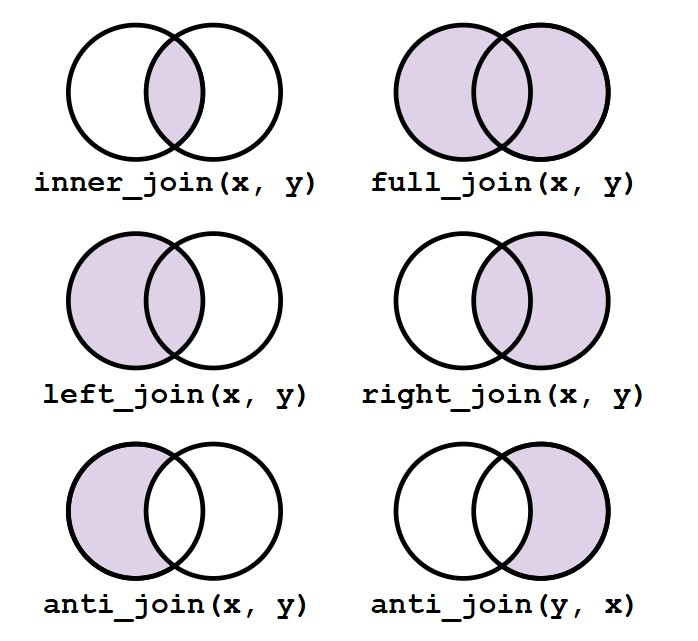
\includegraphics{C:/Users/ASUS/Dropbox/classes/R/book/img/join.jpg}
\caption{Join}
\end{figure}

\begin{Shaded}
\begin{Highlighting}[]
\CommentTok{\# Example datasets}
\NormalTok{data\_grade }\OtherTok{\textless{}{-}} \FunctionTok{data.frame}\NormalTok{(}
  \AttributeTok{subject\_id =} \FunctionTok{seq}\NormalTok{(}\DecValTok{1}\SpecialCharTok{:}\FunctionTok{nrow}\NormalTok{(covid)),    }\CommentTok{\# subject id}
  \AttributeTok{note =} \FunctionTok{sample}\NormalTok{(}\DecValTok{1}\SpecialCharTok{:}\DecValTok{20}\NormalTok{, }\FunctionTok{nrow}\NormalTok{(covid), }\AttributeTok{replace=}\ConstantTok{TRUE}\NormalTok{)                 }\CommentTok{\# Numeric }
\NormalTok{)}

\NormalTok{data\_grade }\OtherTok{\textless{}{-}}\NormalTok{ data\_grade }\SpecialCharTok{\%\textgreater{}\%} 
  \FunctionTok{mutate}\NormalTok{(}\AttributeTok{is\_graduate =} \FunctionTok{ifelse}\NormalTok{(note}\SpecialCharTok{\textgreater{}=}\DecValTok{10}\NormalTok{, }\ConstantTok{TRUE}\NormalTok{, }\ConstantTok{FALSE}\NormalTok{))}

\CommentTok{\# Inner Join: Only matching subject\_id rows}
\NormalTok{join\_data }\OtherTok{\textless{}{-}} \FunctionTok{full\_join}\NormalTok{(covid, data\_grade, }\AttributeTok{by =} \StringTok{"subject\_id"}\NormalTok{)}

\CommentTok{\# Shown results}
\FunctionTok{head}\NormalTok{(join\_data)}
\end{Highlighting}
\end{Shaded}

\begin{verbatim}
## # A tibble: 6 x 23
##   subject_id fake_first_name   fake_last_name gender pan_day test_id clinic_name
##        <dbl> <chr>             <chr>          <chr>    <dbl> <chr>   <chr>      
## 1       1412 jhezane           westerling     female       4 covid   inpatient ~
## 2        533 penny             targaryen      female       7 covid   clinical l~
## 3       9134 grunt             rivers         male         7 covid   clinical l~
## 4       8518 melisandre        swyft          female       8 covid   clinical l~
## 5       8967 SAWADOGO          Laurent Benja~ male         8 covid   emergency ~
## 6      11048 OUATTARA Siguiss~ Sarah          female       8 covid   oncology d~
## # i 16 more variables: result <chr>, demo_group <chr>, age <dbl>,
## #   drive_thru_ind <dbl>, ct_result <dbl>, orderset <dbl>, payor_group <chr>,
## #   patient_class <chr>, col_rec_tat <dbl>, rec_ver_tat <dbl>, age_group <chr>,
## #   age_log <dbl>, age_squarred <dbl>, age_square_root <dbl>, note <int>,
## #   is_graduate <lgl>
\end{verbatim}

\section{Exercises 3}\label{exercises-3}

Try these exercises to practice dplyr functions:

\begin{itemize}
\item
  Import the \textbf{``blood\_storage''} database from the package \textbf{medicaldata}.
\item
  Log-transform the variable \emph{age} in data and save the result as \emph{age.log}in the dataframe.
\item
  Arranging the dataframe using the \emph{age} column.
\item
  Create a new variable called \emph{PVol.squared} with values equal to the square all values in \emph{PVol} (Prostate volume).
  ~
\item
  Create a new variable called \emph{PVol.squared\_root} with values equal to the square root all values in \emph{PVol} (Prostate
  ~volume).
  ~
\item
  Compute the proportion of African American using the column \emph{AA} (0 = ``non‐African-American''; 1 = ``African American'').
\item
  Compute the proportion of African American by Tumor volume (using the variable \emph{TVol}) and the mean and variance of the column \emph{age}.
\item
  Filter out the records for which \emph{(PreopPSA \textgreater= 10)} and \emph{(Recurrence == 0)} using the \textbf{filter} function.
\item
  Create a new column called \emph{subject\_id} and merge the \textbf{``covid''} database with the \textbf{``blood\_storage''} using the newly created column.
\end{itemize}

This lesson introduces essential dplyr functions for data manipulation in R. Try the exercises and explore the dataset further! 🚀

\chapter{Data Visualization with ggplot}\label{data-visualization-with-ggplot}

\section{Overview}\label{overview}

The \texttt{ggplot2} package is one of the most powerful and flexible tools for creating complex, multi-layered graphics in \textbf{R}. It implements the Grammar of Graphics, a framework that breaks down plots into semantic components such as layers, scales, and themes.

\section{Basic Concepts}\label{basic-concepts}

\begin{itemize}
\tightlist
\item
  \textbf{Aesthetic Mappings (\texttt{aes()})}: Defines how data variables are mapped to visual properties like color, size, and shape.
\item
  \textbf{Geometries (\texttt{geom\_*})}: Defines the type of plot, such as points (\texttt{geom\_point}), lines (\texttt{geom\_line}), and bars (\texttt{geom\_bar}).
\item
  \textbf{Layers}: Multiple geometries can be added to a plot.
\item
  \textbf{Scales and Coordinate Systems}: Allows control over appearance.
\item
  \textbf{Themes}: Adjust non-data elements like background and grid lines.
\end{itemize}

\section{Scatter Plot}\label{scatter-plot}

\subsection{Basic Scatter Plot}\label{basic-scatter-plot}

\begin{Shaded}
\begin{Highlighting}[]
\CommentTok{\# Load libraries}
\FunctionTok{library}\NormalTok{(dplyr)}
\FunctionTok{library}\NormalTok{(ggplot2)}
\FunctionTok{library}\NormalTok{(readr)}

\CommentTok{\# Load the COVID{-}19 dataset}
\NormalTok{covid\_data }\OtherTok{\textless{}{-}} \FunctionTok{read\_csv}\NormalTok{(}\StringTok{"country\_wise\_latest.csv"}\NormalTok{)}
\end{Highlighting}
\end{Shaded}

\begin{verbatim}
## Rows: 187 Columns: 15
## -- Column specification --------------------------------------------------------
## Delimiter: ","
## chr  (2): Country/Region, WHO Region
## dbl (13): Confirmed, Deaths, Recovered, Active, New cases, New deaths, New r...
## 
## i Use `spec()` to retrieve the full column specification for this data.
## i Specify the column types or set `show_col_types = FALSE` to quiet this message.
\end{verbatim}

\begin{Shaded}
\begin{Highlighting}[]
\CommentTok{\#View(covid\_data)}

\CommentTok{\# Create the scatter plot}
\FunctionTok{ggplot}\NormalTok{(covid\_data, }\CommentTok{\# The data frame containing the COVID{-}19 data}
       \FunctionTok{aes}\NormalTok{(}\AttributeTok{x =} \StringTok{\textasciigrave{}}\AttributeTok{Recovered / 100 Cases}\StringTok{\textasciigrave{}}\NormalTok{, }\CommentTok{\# Variable for the x{-}axis (Recovered cases per 100)}
           \AttributeTok{y =} \StringTok{\textasciigrave{}}\AttributeTok{Deaths / 100 Cases}\StringTok{\textasciigrave{}}\NormalTok{)) }\SpecialCharTok{+} \CommentTok{\# Variable for the y{-}axis (Deaths per 100 cases)}
  \FunctionTok{geom\_point}\NormalTok{(}\AttributeTok{color =} \StringTok{\textquotesingle{}navy\textquotesingle{}}\NormalTok{) }\SpecialCharTok{+} \CommentTok{\# Add points to the plot, colored navy}
  \FunctionTok{labs}\NormalTok{(}\AttributeTok{title =} \StringTok{"Recovered vs. Deaths of Covid19"}\NormalTok{, }\CommentTok{\# Set the plot title}
       \AttributeTok{x =} \StringTok{"Recovered (per 100 cases)"}\NormalTok{, }\CommentTok{\# Set the x{-}axis label}
       \AttributeTok{y =} \StringTok{"Deaths (per 100 cases)"}\NormalTok{) }\SpecialCharTok{+} \CommentTok{\# Set the y{-}axis label}
  \FunctionTok{theme\_minimal}\NormalTok{() }\CommentTok{\# Use a minimal theme for a cleaner look}
\end{Highlighting}
\end{Shaded}

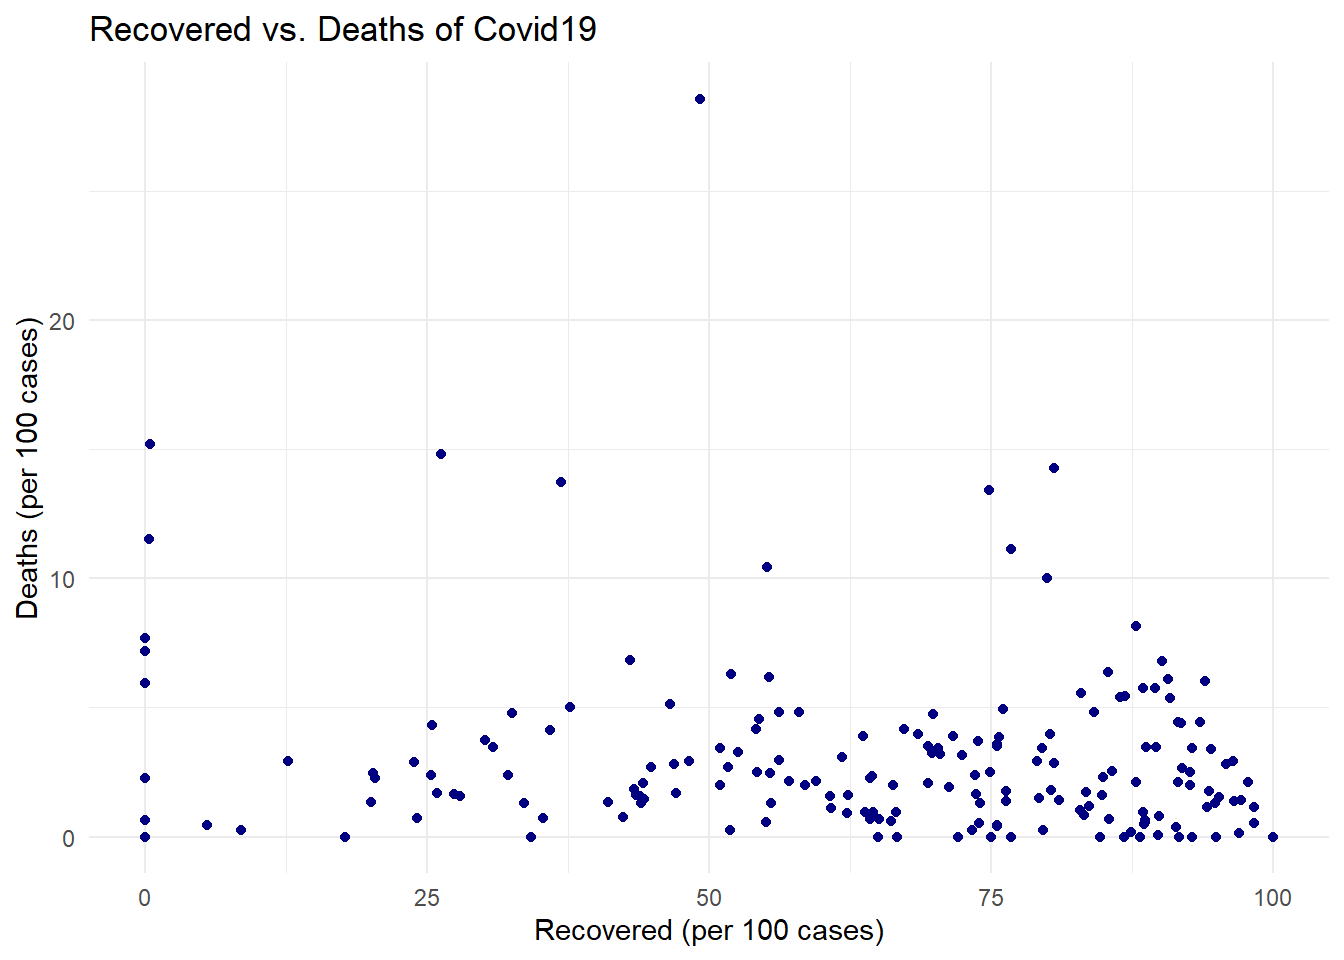
\includegraphics{_main_files/figure-latex/unnamed-chunk-22-1.pdf}

\subsection{Scatter Plots and Line Plots}\label{scatter-plots-and-line-plots}

\begin{Shaded}
\begin{Highlighting}[]
\CommentTok{\# Create the scatter plot with a smooth line}
\FunctionTok{ggplot}\NormalTok{(covid\_data, }\CommentTok{\# The data frame containing the COVID{-}19 data}
       \FunctionTok{aes}\NormalTok{(}\AttributeTok{x =} \StringTok{\textasciigrave{}}\AttributeTok{Recovered / 100 Cases}\StringTok{\textasciigrave{}}\NormalTok{, }\CommentTok{\# Variable for the x{-}axis (Recovered cases per 100)}
           \AttributeTok{y =} \StringTok{\textasciigrave{}}\AttributeTok{Deaths / 100 Cases}\StringTok{\textasciigrave{}}\NormalTok{)) }\SpecialCharTok{+} \CommentTok{\# Variable for the y{-}axis (Deaths per 100 cases)}
  \FunctionTok{geom\_point}\NormalTok{(}\AttributeTok{color =} \StringTok{\textquotesingle{}navy\textquotesingle{}}\NormalTok{) }\SpecialCharTok{+} \CommentTok{\# Add points to the plot, colored navy}
  \FunctionTok{geom\_smooth}\NormalTok{(}\AttributeTok{method =} \StringTok{"lm"}\NormalTok{, }\CommentTok{\# Add a smooth line, using a linear model ("lm")}
              \AttributeTok{color =} \StringTok{"black"}\NormalTok{, }\CommentTok{\# Set the line color to black}
              \AttributeTok{se =} \ConstantTok{TRUE}\NormalTok{) }\SpecialCharTok{+} \CommentTok{\# Display the standard error around the line}
  \FunctionTok{labs}\NormalTok{(}\AttributeTok{title =} \StringTok{"Recovered vs. Deaths of Covid19"}\NormalTok{, }\CommentTok{\# Set the plot title}
       \AttributeTok{x =} \StringTok{"Recovered (per 100 cases)"}\NormalTok{, }\CommentTok{\# Set the x{-}axis label}
       \AttributeTok{y =} \StringTok{"Deaths (per 100 cases)"}\NormalTok{) }\SpecialCharTok{+} \CommentTok{\# Set the y{-}axis label}
  \FunctionTok{theme\_minimal}\NormalTok{() }\CommentTok{\# Use a minimal theme for a cleaner look}
\end{Highlighting}
\end{Shaded}

\begin{verbatim}
## `geom_smooth()` using formula = 'y ~ x'
\end{verbatim}

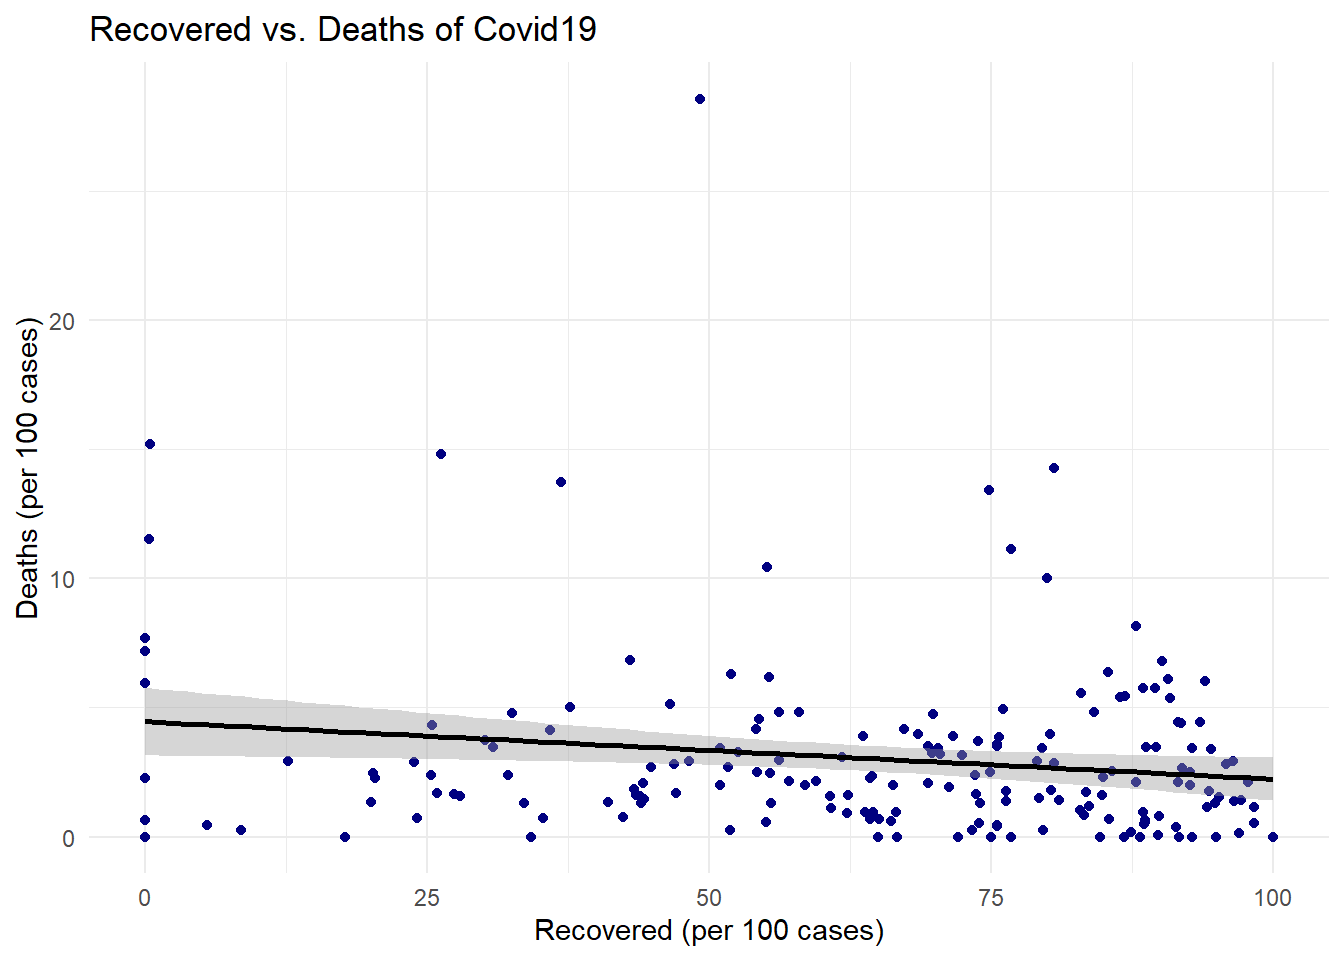
\includegraphics{_main_files/figure-latex/unnamed-chunk-23-1.pdf}

\section{Exercise 1: Customizing Your First Plot}\label{exercise-1-customizing-your-first-plot}

\textbf{Objective}: Create a scatter plot showing the relationship between \texttt{proportion\_of\_active} and \texttt{proportion\_of\_recovery}. Customize the plot:
- Create a new variable (using the function \texttt{mutate}of the package \texttt{dplyr}) named \texttt{proportion\_of\_active} = \texttt{Active}/\texttt{Confirmed}.
- Create a new variable (using the function \texttt{mutate}of the package \texttt{dplyr}) named \texttt{proportion\_of\_recovery} = \texttt{Recovered}/\texttt{Confirmed}.
- Change the color of the points to ``darkturquoise'' \href{https://sape.inf.usi.ch/quick-reference/ggplot2/colour}{(see list of color names)}
- Adjust the size of the points to 3.
- Use triangles for the point shapes.
- Add the regression line with the confidence interval estimate.

\section{Bar Plots and Histograms}\label{bar-plots-and-histograms}

\subsection{Histogram:}\label{histogram}

\begin{Shaded}
\begin{Highlighting}[]
\CommentTok{\# Create the histogram}
\FunctionTok{ggplot}\NormalTok{(covid\_data, }\CommentTok{\# The data frame containing the COVID{-}19 data}
       \FunctionTok{aes}\NormalTok{(}\AttributeTok{x =} \StringTok{\textasciigrave{}}\AttributeTok{New deaths}\StringTok{\textasciigrave{}}\NormalTok{)) }\SpecialCharTok{+} \CommentTok{\# Variable for the x{-}axis (New deaths)}
  \FunctionTok{geom\_histogram}\NormalTok{(}\AttributeTok{fill =} \StringTok{"skyblue"}\NormalTok{, }\CommentTok{\# Fill the bars with skyblue}
                 \AttributeTok{color =} \StringTok{"black"}\NormalTok{) }\SpecialCharTok{+} \CommentTok{\# Set the bar outline color to black}
  \FunctionTok{labs}\NormalTok{(}\AttributeTok{title =} \StringTok{"Number of deaths of COVID{-}19"}\NormalTok{, }\CommentTok{\# Set the plot title}
       \AttributeTok{x =} \StringTok{"Number of deaths"}\NormalTok{, }\CommentTok{\# Set the x{-}axis label}
       \AttributeTok{y =} \StringTok{"Frequency"}\NormalTok{) }\SpecialCharTok{+} \CommentTok{\# Set the y{-}axis label}
  \FunctionTok{theme\_minimal}\NormalTok{() }\CommentTok{\# Use a minimal theme for a cleaner look}
\end{Highlighting}
\end{Shaded}

\begin{verbatim}
## `stat_bin()` using `bins = 30`. Pick better value with `binwidth`.
\end{verbatim}

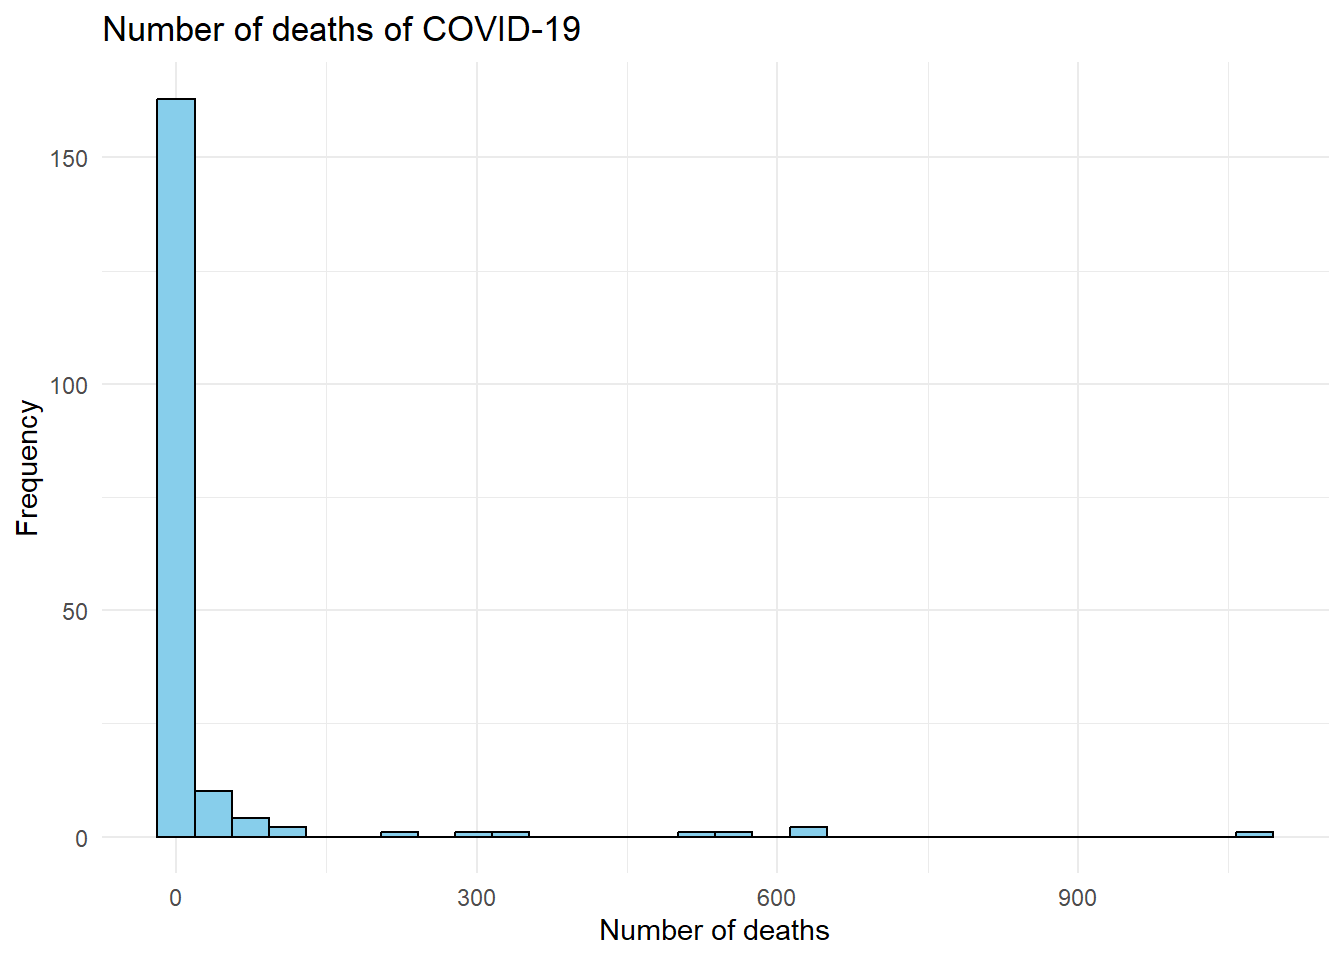
\includegraphics{_main_files/figure-latex/unnamed-chunk-24-1.pdf}

\subsection{Bar Plot}\label{bar-plot}

\begin{Shaded}
\begin{Highlighting}[]
\CommentTok{\# Calculate mean recovery rates by region and create bar plot}
\NormalTok{covid\_data }\SpecialCharTok{\%\textgreater{}\%} \CommentTok{\# Start with the COVID{-}19 data}
  \FunctionTok{group\_by}\NormalTok{(}\StringTok{\textasciigrave{}}\AttributeTok{WHO Region}\StringTok{\textasciigrave{}}\NormalTok{) }\SpecialCharTok{\%\textgreater{}\%} \CommentTok{\# Group the data by WHO Region}
  \FunctionTok{summarise}\NormalTok{(}\AttributeTok{mean\_recovery =} \FunctionTok{mean}\NormalTok{(}\StringTok{\textasciigrave{}}\AttributeTok{Recovered / 100 Cases}\StringTok{\textasciigrave{}}\NormalTok{, }\AttributeTok{na.rm =} \ConstantTok{TRUE}\NormalTok{)) }\SpecialCharTok{\%\textgreater{}\%} \CommentTok{\# Calculate the mean recovery rate for each region, removing NA values}
  \FunctionTok{ggplot}\NormalTok{(}\FunctionTok{aes}\NormalTok{(}\AttributeTok{y =}\NormalTok{ mean\_recovery, }\CommentTok{\# Set the y{-}axis to the mean recovery rate}
             \AttributeTok{x =} \StringTok{\textasciigrave{}}\AttributeTok{WHO Region}\StringTok{\textasciigrave{}}\NormalTok{, }\CommentTok{\# Set the x{-}axis to the WHO Region}
             \AttributeTok{fill =} \StringTok{\textasciigrave{}}\AttributeTok{WHO Region}\StringTok{\textasciigrave{}}\NormalTok{)) }\SpecialCharTok{+} \CommentTok{\# Fill the bars with different colors based on the region}
  \FunctionTok{geom\_bar}\NormalTok{(}\AttributeTok{stat =} \StringTok{"identity"}\NormalTok{, }\CommentTok{\# Use "identity" because we\textquotesingle{}ve already calculated the means}
           \AttributeTok{color =} \StringTok{"black"}\NormalTok{) }\SpecialCharTok{+} \CommentTok{\# Set the bar outline color to black}
  \FunctionTok{labs}\NormalTok{(}\AttributeTok{title =} \StringTok{"Mean recovered by region"}\NormalTok{, }\CommentTok{\# Set the plot title}
       \AttributeTok{x =} \StringTok{"WHO Region"}\NormalTok{, }\CommentTok{\# Set the x{-}axis label}
       \AttributeTok{y =} \StringTok{"Mean Recovered (per 100 cases)"}\NormalTok{) }\SpecialCharTok{+} \CommentTok{\# Set the y{-}axis label}
  \FunctionTok{theme\_minimal}\NormalTok{() }\SpecialCharTok{+} \CommentTok{\# Use a minimal theme for a cleaner look}
  \FunctionTok{theme}\NormalTok{(}\AttributeTok{axis.text.x =} \FunctionTok{element\_text}\NormalTok{(}\AttributeTok{angle =} \DecValTok{45}\NormalTok{, }\AttributeTok{hjust =} \DecValTok{1}\NormalTok{)) }\CommentTok{\# Rotate x{-}axis labels for better readability}
\end{Highlighting}
\end{Shaded}

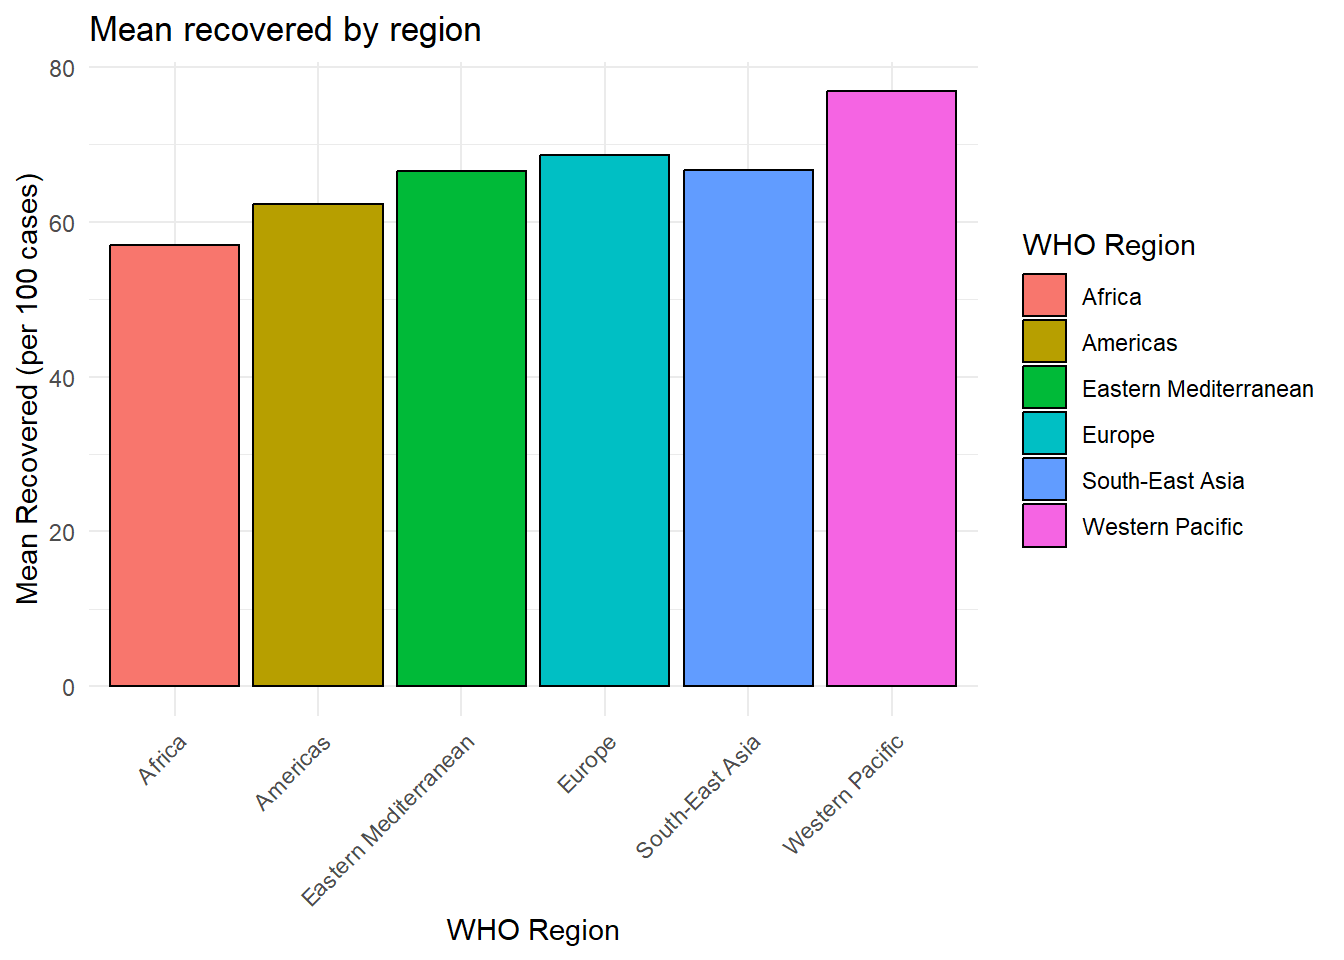
\includegraphics{_main_files/figure-latex/unnamed-chunk-25-1.pdf}

\begin{Shaded}
\begin{Highlighting}[]
\FunctionTok{library}\NormalTok{(medicaldata) }\CommentTok{\# For the covid\_testing dataset}

\CommentTok{\# Load the covid\_testing dataset}
\NormalTok{testing\_data }\OtherTok{\textless{}{-}}\NormalTok{ medicaldata}\SpecialCharTok{::}\NormalTok{covid\_testing}

\CommentTok{\# Analyze test results by gender and create bar plot}
\NormalTok{testing\_data }\SpecialCharTok{\%\textgreater{}\%}
  \FunctionTok{group\_by}\NormalTok{(gender, result) }\SpecialCharTok{\%\textgreater{}\%} \CommentTok{\# Group the data by gender and test result}
  \FunctionTok{summarise}\NormalTok{(}\AttributeTok{age\_moyen =} \FunctionTok{mean}\NormalTok{(age, }\AttributeTok{na.rm=}\ConstantTok{TRUE}\NormalTok{)) }\SpecialCharTok{\%\textgreater{}\%} \CommentTok{\# Count the number of individuals in each group}
  \FunctionTok{ungroup}\NormalTok{() }\SpecialCharTok{\%\textgreater{}\%} \CommentTok{\# Ungroup the data for plotting}
  \FunctionTok{ggplot}\NormalTok{(}\FunctionTok{aes}\NormalTok{(}\AttributeTok{y =}\NormalTok{ age\_moyen, }\CommentTok{\# Set the y{-}axis to the mean age}
             \AttributeTok{x =}\NormalTok{ result, }\CommentTok{\# Set the x{-}axis to the test result}
             \AttributeTok{fill =}\NormalTok{ gender)) }\SpecialCharTok{+} \CommentTok{\# Fill the bars with different colors based on gender}
  \FunctionTok{geom\_bar}\NormalTok{(}\AttributeTok{stat =} \StringTok{"identity"}\NormalTok{, }\CommentTok{\# Use "identity" because we\textquotesingle{}ve already calculated the counts}
           \AttributeTok{color =} \StringTok{"black"}\NormalTok{, }\CommentTok{\# Set the bar outline color to black}
           \AttributeTok{position =} \StringTok{"dodge"}\NormalTok{) }\SpecialCharTok{+} \CommentTok{\# Place bars for different genders side{-}by{-}side}
  \FunctionTok{labs}\NormalTok{(}\AttributeTok{title =} \StringTok{"COVID{-}19 Test Results by Gender"}\NormalTok{, }\CommentTok{\# Set the plot title}
       \AttributeTok{x =} \StringTok{"Result of the COVID{-}19 test"}\NormalTok{, }\CommentTok{\# Set the x{-}axis label}
       \AttributeTok{y =} \StringTok{"Number of Individuals"}\NormalTok{, }\CommentTok{\# Set the y{-}axis label}
       \AttributeTok{fill =} \StringTok{"Gender"}\NormalTok{) }\SpecialCharTok{+} \CommentTok{\# Set the legend title}
  \FunctionTok{theme\_minimal}\NormalTok{() }\SpecialCharTok{+} \CommentTok{\# Use a minimal theme for a cleaner look}
  \FunctionTok{theme}\NormalTok{(}\AttributeTok{axis.text.x =} \FunctionTok{element\_text}\NormalTok{(}\AttributeTok{angle =} \DecValTok{45}\NormalTok{, }\AttributeTok{hjust =} \DecValTok{1}\NormalTok{)) }\CommentTok{\# Rotate x{-}axis labels for better readability}
\end{Highlighting}
\end{Shaded}

\begin{verbatim}
## `summarise()` has grouped output by 'gender'. You can override using the
## `.groups` argument.
\end{verbatim}

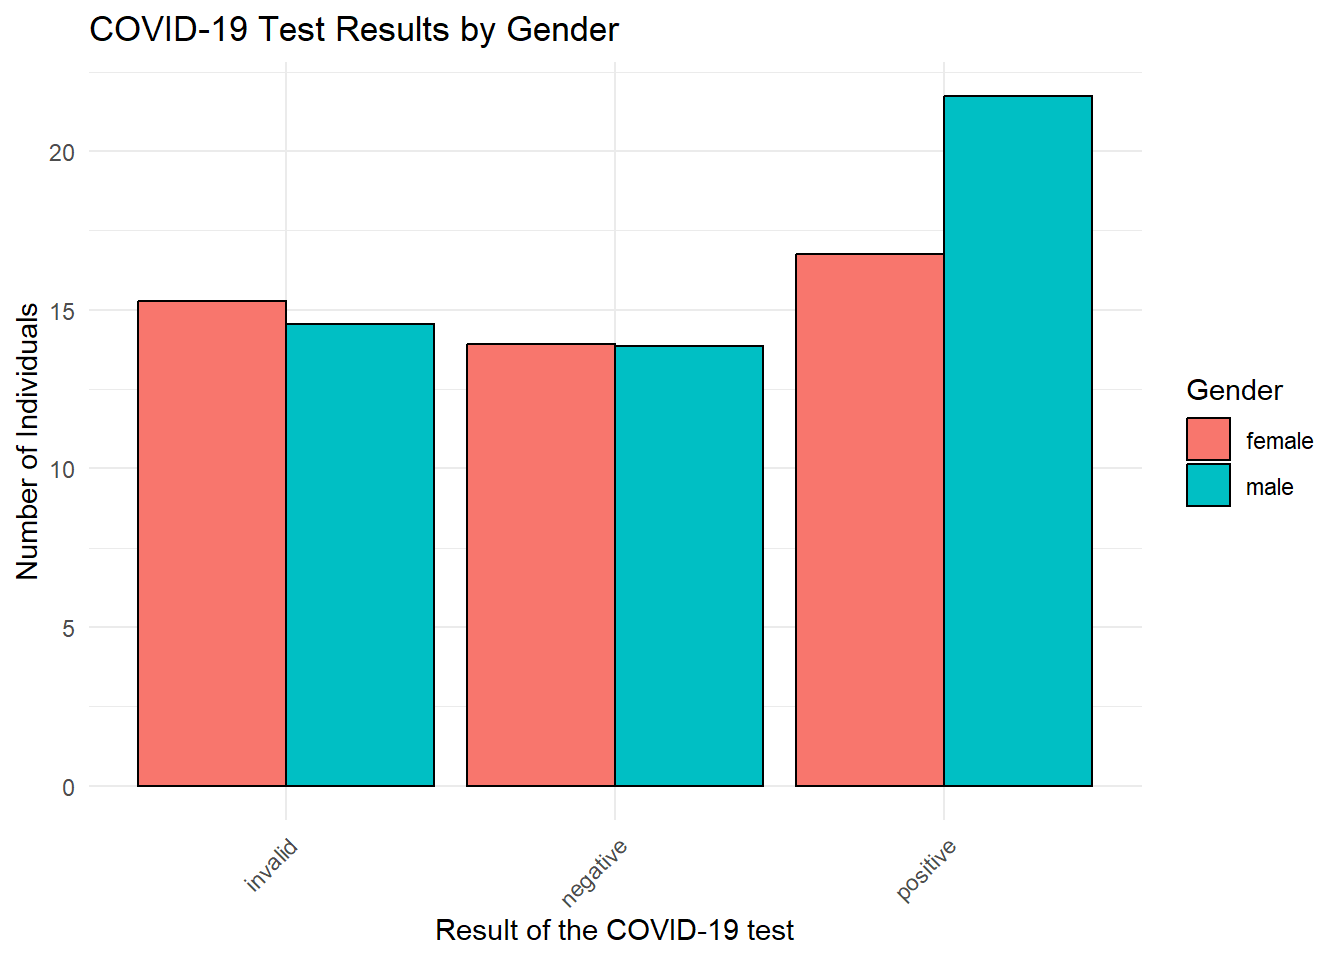
\includegraphics{_main_files/figure-latex/unnamed-chunk-26-1.pdf}

\section{Exercise 3: Creating Histograms and Bar Plots}\label{exercise-3-creating-histograms-and-bar-plots}

\begin{itemize}
\tightlist
\item
  Import the \textbf{blood\_storage} database from the \textbf{medicaldata} package.
\item
  Log-transform the variable \textbf{age} in the data and save the result as \textbf{age.log} in the dataframe.
\item
  Compare the histograms of the \textbf{age} and \textbf{age.log} variables and comment on the distribution.
\item
  Create a bar plot of the mean \textbf{PVol} by aggregating by race (use the \textbf{AA} variable).
\item
  Create a bar plot of the mean \textbf{PVol} by aggregating by the volume of the tumor (use the **TVol\} variable).
\end{itemize}

  \bibliography{book.bib,packages.bib}

\end{document}
